\documentclass[11pt]{article}

% Change "review" to "final" for the camera-ready version.
% Change to "preprint" for a non-anonymous version with page numbers.
\usepackage[final]{acl}

% Standard package includes
\usepackage{times}
\usepackage{latexsym}
\usepackage[T1]{fontenc}
\usepackage[utf8]{inputenc}
\usepackage{microtype}
\usepackage{inconsolata}
\usepackage{graphicx}

% Additional packages we use
\usepackage{booktabs}
\usepackage{multirow}
\usepackage{array}
\usepackage{amsmath}
\usepackage{amssymb}
\usepackage{xcolor}
\usepackage{caption}
\usepackage{tikz}
\usetikzlibrary{positioning, arrows.meta, fit, calc, shapes.geometric, backgrounds}

% Allow URLs to break across lines in the bibliography
\usepackage{url}
\Urlmuskip=0mu plus 1mu\relax
\def\UrlBreaks{\do\/\do-\do\.\do\_\do\?\do\&\do\=\do\#\do\+\do\@\do\:}

% Keep tables inside their section: prevents appendix floats from drifting
% into other sections and from stacking up at the end of the paper.
\usepackage[section]{placeins}

% Make tables a bit more compact
\renewcommand{\arraystretch}{1.05}

\title{Beyond the Login: Continuous Behavioral Authorship Verification for LLM Agent Sessions}

% =========================================================================
% IMPORTANT: ACL/AACL Rolling Review is DOUBLE-BLIND.
% Keep the author line as "Anonymous ACL submission" during review.
% Submitting with real names = desk rejection before review.
% After acceptance, comment out the anonymous line and uncomment the
% camera-ready block below.
% =========================================================================

% --- Review submission (re-activate for any future anonymous submission) ---
% \author{Anonymous ACL submission}

% --- Camera-ready ---
\author{Muskan Sharma \\
  Independent Researcher \\
  \texttt{muskankalonia@gmail.com} \\\And
  Seba Susan \\
  Dept.\ of Information Technology \\
  Delhi Technological University \\
  \texttt{sebasusan@dce.ac.in} \\}

\begin{document}
\maketitle
\begin{abstract}
LLM agents now operate as a privileged application layer, with access to mail, files and MCP-connected tools, yet they have no built-in way to verify that the person typing into an already-signed-in session is still the legitimate user. This identity gap aligns with OWASP LLM06 (Excessive Agency), Agentic ASI03 (Identity and Privilege Abuse), and NIST guidance on AI risk management, but whether it is closable from user text alone is largely open. We build a profile-query authorship verification benchmark on WildChat-1M and PAN-20 regrouped per author, with author-disjoint 60/20/20 splits across three seeds. We train contrastive bi-encoders with triplet margin loss on DistilBERT, BERT, MiniLM-L6 and ELECTRA, under 100\% random imposters or a 50/30/20 mix of random, semi-hard and hard imposters mined by TF-IDF. Models trained on random imposters look strong (ROC-AUC above 0.95) but drop by around 10 points on WildChat against topic-similar imposters, suggesting they rely on topic and vocabulary rather than writing style only. Our contribution is to expose and quantify this failure mode and to provide a reproducible hardness-stratified benchmark; applying established hardness-aware training as a controlled mitigation closes most of the gap, lifting TAR@FAR=1\% on WildChat Hard from around 6--7\% to 20--22\% for BERT and DistilBERT with median messages-to-detect of one, and the same direction holds under a secondary SBERT miner. We release the benchmark construction and evaluation code.
\end{abstract}

\section{Introduction}
\label{sec:intro}

LLM agents are quietly becoming one of the most privileged pieces of software on a user's machine. With protocols like Model Context Protocol \citep{anthropic2024mcp} an agent can be connected to tools that send the user's mail, push commits, edit files in the user's workspace and run a shell command, all on the basis of a few words typed into a chat box.\footnote{Our benchmark-construction scripts and evaluation code are available at \url{https://github.com/Muskankalonia/beyond-the-login-continuous-authorship-verification-LLM}.} While these capabilities substantially improve user productivity, they also introduce a persistent authentication problem: once an agent session has been authenticated, subsequent actions are typically authorized solely on the basis of continued session access. Consequently, any individual with access to an already authenticated interface—whether through device sharing, session exposure, or workstation compromise—may issue commands with the same privileges as the legitimate user. Existing agent architectures generally lack mechanisms for continuously verifying that the active operator remains consistent with the user who originally authenticated the session. Behavioral authorship verification refers to the task of determining whether two text segments originate from the same author based on patterns in their writing behavior across interaction histories, rather than relying solely on static stylistic features of isolated documents.

Many surrounding layers already perform some form of identity or authorization check: the operating system authenticates the user at login or unlock, Multi-Factor Authentication (MFA) may be required for sensitive services, and browser or OAuth tokens authorize access to external applications. The LLM agent layer, however, usually has no equivalent check once a session is already open. The security community has identified related risks: the OWASP Top 10 for LLM Applications \citep{owasp2025llm} lists LLM06: Excessive Agency, the OWASP Top 10 for Agentic Applications \citep{owasp2026agentic} identifies ASI03: Identity and Privilege Abuse, MITRE ATT\&CK lists Impersonation \citep{mitre_t1656} as an established adversary technique, and NIST's AI Risk Management Framework \citep{nist2023airmf} emphasizes governance and accountability for AI systems. These frameworks motivate the risk, but they do not answer whether the problem is technically solvable at the agent layer using only the signal the agent reliably has: the text the user has typed. This paper investigates that question and, additionally, examines the amount of interaction context required for a verifier to make reliable authorship verification decisions.

We model continuous authorship verification as a representation-learning problem over interaction text. Given a reference \emph{profile} consisting of previously observed user messages and an incoming \emph{query} message, a text encoder maps both inputs into a shared embedding space. Profile-level and query-level representations are then compared using cosine similarity to estimate whether the incoming message is consistent with the enrolled user identity. We instantiate this idea with a contrastive bi-encoder trained using triplet margin loss. The model performs very well when the imposter corresponds to a uniformly random alternative user: on the random test regime, ROC-AUC rises above 0.9 even for MiniLM-L6, a 22.71M-parameter encoder. At first glance, the problem appears close to solved.

But a uniformly random imposter is not the hardest adversary an LLM agent may face. A real imposter may share a workplace, family, or social circle with the user; they may know the same projects, codebases, or clients; and the topics they discuss may overlap substantially with those of the legitimate user. When we replace the random imposter with another real user mined for topical similarity using TF-IDF over character and word $n$-grams, performance drops sharply: on WildChat, ROC-AUC falls by about 10 points on the hardest 5\% of imposters for several encoders. The model that looked excellent on random imposters becomes much less reliable against topic-similar imposters, suggesting that it relies partly on topic and vocabulary rather than writing style alone. This topic-vs-style gap is the empirical core of the paper.

Because the failure mode is security-relevant, we evaluate at security operating points rather than relying only on ROC-AUC. We report \textbf{TAR@FAR=1\%} (fraction of genuine users accepted at a fixed 1\% imposter false-accept rate), \textbf{FAR@FRR=1\%} (the symmetric metric), EER, the robustness gap between random and hard imposters, and streaming metrics over the first three query messages (catch@3, median messages-to-detect). The full metric list and security interpretation is in Section~\ref{sec:expsetup}. Our key finding is that replacing purely random training negatives with a 50/30/20 mix of random, semi-hard and hard imposters substantially reduces the random-to-hard robustness gap, especially on WildChat: TAR@FAR=1\% on WildChat Hard rises from 6-7\% under random-only training to 20-22\% under hardness-aware training for BERT and DistilBERT, while the median messages-to-detect remains one. We build this benchmark from WildChat-1M \citep{zhao2024wildchat} as the primary dataset and PAN-20 \citep{bevendorff2020overview} regrouped at the author level as a secondary, with author-disjoint 60/20/20 splits across three seeds and a 70/30 profile-query split within each author. We release the benchmark construction scripts and evaluation code.

\noindent\textbf{Contributions.} We do not propose a new negative-sampling algorithm; hard-negative mining is well established in metric learning and dense retrieval \citep{schroff2015facenet,xiong2021ance,robinson2021hard}. Instead, we (i) identify a security-relevant evaluation gap: random-imposter tests overestimate robustness by letting continuous authorship verifiers exploit topic and vocabulary shortcuts; (ii) release a reproducible, hardness-stratified profile-query benchmark with author-disjoint splits and security-oriented metrics (TAR@FAR, FAR@FRR, EER, catch@3, median messages-to-detect); and (iii) show that hardness-aware training, used as a controlled mitigation, narrows but does not close the gap across four encoders, two datasets, strict operating points, and two independent hardness miners.

\section{Threat Model}
\label{sec:threat}

\begin{figure*}[t]
\centering
\resizebox{0.95\textwidth}{!}{% System-overview block diagram for "Beyond the Login".
% Drop into draft.tex with:
%   \begin{figure*}[t]
%     \centering
%     \resizebox{0.95\textwidth}{!}{% System-overview block diagram for "Beyond the Login".
% Drop into draft.tex with:
%   \begin{figure*}[t]
%     \centering
%     \resizebox{0.95\textwidth}{!}{% System-overview block diagram for "Beyond the Login".
% Drop into draft.tex with:
%   \begin{figure*}[t]
%     \centering
%     \resizebox{0.95\textwidth}{!}{\input{figures/system_overview}}
%     \caption{...}
%     \label{fig:system_overview}
%   \end{figure*}
%
% Requires (already in draft.tex):
%   \usepackage{tikz}
%   \usetikzlibrary{positioning, arrows.meta, fit, calc, shapes.geometric, backgrounds}

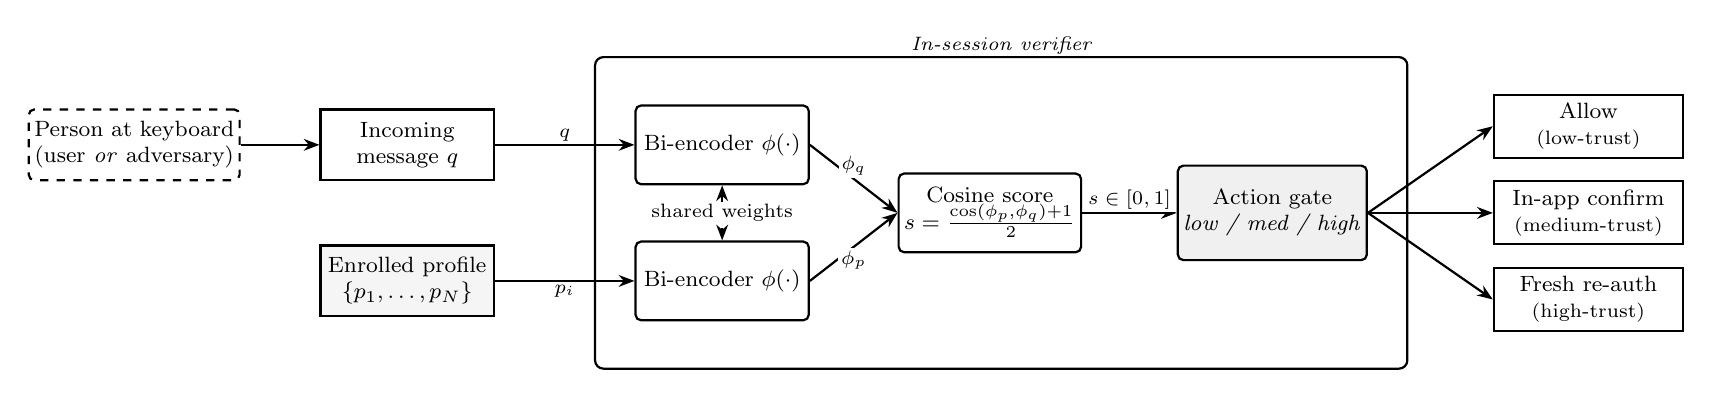
\begin{tikzpicture}[
    font=\footnotesize,
    >={Stealth[length=2mm]},
    block/.style={
        draw, thick, rounded corners=2pt,
        minimum width=22mm, minimum height=10mm,
        align=center, inner sep=2pt, fill=white
    },
    io/.style={
        draw, thick,
        minimum width=22mm, minimum height=9mm,
        align=center, inner sep=2pt, fill=white
    },
    profilebox/.style={
        draw, thick,
        minimum width=22mm, minimum height=9mm,
        align=center, inner sep=2pt, fill=gray!8
    },
    gate/.style={
        draw, thick, rounded corners=2pt,
        minimum width=22mm, minimum height=12mm,
        align=center, inner sep=2pt, fill=gray!12
    },
    actor/.style={
        draw, thick, dashed, rounded corners=2pt,
        minimum width=22mm, minimum height=9mm,
        align=center, inner sep=2pt
    },
    outcome/.style={
        draw, thick,
        minimum width=24mm, minimum height=8mm,
        align=center, inner sep=2pt, fill=white
    },
    arrow/.style={->, thick},
    midlabel/.style={font=\scriptsize, midway, fill=white, inner sep=1pt}
]

% --- Actor on the left ---
\node[actor] (typist) at (0,0) {Person at keyboard\\(user \emph{or} adversary)};

% --- Incoming message and stored profile ---
\node[io, right=10mm of typist] (msg) {Incoming\\message $q$};
\node[profilebox, below=8mm of msg] (profile) {Enrolled profile\\$\{p_1,\dots,p_N\}$};

% --- Shared bi-encoder: two instances of the SAME encoder (shared weights) ---
\node[block] (encq) at ($(msg) + (40mm,0)$)
    {Bi-encoder $\phi(\cdot)$};
\node[block] (encp) at ($(profile) + (40mm,0)$)
    {Bi-encoder $\phi(\cdot)$};
\draw[<->, thick, dashed] (encq.south) -- node[midlabel]{\scriptsize shared weights} (encp.north);

% --- Cosine score and action gate ---
\node[block] (score) at ($(encq)!0.5!(encp) + (34mm,0)$)
    {Cosine score\\$s=\tfrac{\cos(\phi_p,\phi_q)+1}{2}$};
\node[gate, right=12mm of score] (gateNode)
    {Action gate\\\textit{low / med / high}};

% --- Outcomes: wider gap so arrow labels do not overlap ---
\node[outcome] (allow)   at ($(gateNode.east) + (28mm, 11mm)$) {Allow\\\scriptsize(low-trust)};
\node[outcome] (confirm) at ($(gateNode.east) + (28mm,  0mm)$) {In-app confirm\\\scriptsize(medium-trust)};
\node[outcome] (block)   at ($(gateNode.east) + (28mm,-11mm)$) {Fresh re-auth\\\scriptsize(high-trust)};

% --- Typist to message ---
\draw[arrow] (typist.east) -- (msg.west);

% --- Message and profile each into their own copy of the shared encoder ---
\draw[arrow] (msg.east)     -- node[midlabel, above]{$q$}   (encq.west);
\draw[arrow] (profile.east) -- node[midlabel, below]{$p_i$} (encp.west);

% --- Each encoder output to cosine; cosine to gate ---
\draw[arrow] (encq.east) -- node[midlabel, above]{$\phi_q$} (score.west);
\draw[arrow] (encp.east) -- node[midlabel, below]{$\phi_p$} (score.west);
\draw[arrow] (score.east) -- node[midlabel, above]{$s\in[0,1]$}    (gateNode.west);

% --- Gate to outcomes (no on-arrow labels; tiers now inside outcome boxes) ---
\draw[arrow] (gateNode.east) -- (allow.west);
\draw[arrow] (gateNode.east) -- (confirm.west);
\draw[arrow] (gateNode.east) -- (block.west);

% --- Bounding box around verifier ---
\begin{scope}[on background layer]
    \node[
        fit=(encq)(encp)(score)(gateNode),
        draw, thick, rounded corners=3pt,
        inner xsep=5mm, inner ysep=6mm,
        label={[anchor=south, font=\scriptsize\itshape, yshift=-1mm]north:In-session verifier}
    ] (verifier) {};
\end{scope}

\end{tikzpicture}
}
%     \caption{...}
%     \label{fig:system_overview}
%   \end{figure*}
%
% Requires (already in draft.tex):
%   \usepackage{tikz}
%   \usetikzlibrary{positioning, arrows.meta, fit, calc, shapes.geometric, backgrounds}

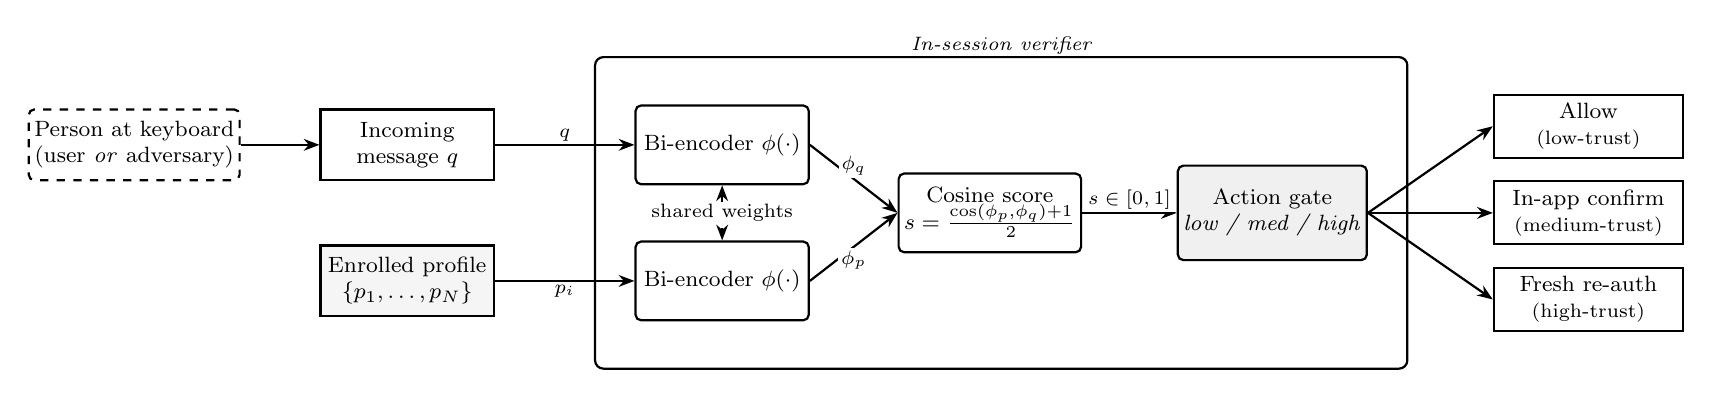
\begin{tikzpicture}[
    font=\footnotesize,
    >={Stealth[length=2mm]},
    block/.style={
        draw, thick, rounded corners=2pt,
        minimum width=22mm, minimum height=10mm,
        align=center, inner sep=2pt, fill=white
    },
    io/.style={
        draw, thick,
        minimum width=22mm, minimum height=9mm,
        align=center, inner sep=2pt, fill=white
    },
    profilebox/.style={
        draw, thick,
        minimum width=22mm, minimum height=9mm,
        align=center, inner sep=2pt, fill=gray!8
    },
    gate/.style={
        draw, thick, rounded corners=2pt,
        minimum width=22mm, minimum height=12mm,
        align=center, inner sep=2pt, fill=gray!12
    },
    actor/.style={
        draw, thick, dashed, rounded corners=2pt,
        minimum width=22mm, minimum height=9mm,
        align=center, inner sep=2pt
    },
    outcome/.style={
        draw, thick,
        minimum width=24mm, minimum height=8mm,
        align=center, inner sep=2pt, fill=white
    },
    arrow/.style={->, thick},
    midlabel/.style={font=\scriptsize, midway, fill=white, inner sep=1pt}
]

% --- Actor on the left ---
\node[actor] (typist) at (0,0) {Person at keyboard\\(user \emph{or} adversary)};

% --- Incoming message and stored profile ---
\node[io, right=10mm of typist] (msg) {Incoming\\message $q$};
\node[profilebox, below=8mm of msg] (profile) {Enrolled profile\\$\{p_1,\dots,p_N\}$};

% --- Shared bi-encoder: two instances of the SAME encoder (shared weights) ---
\node[block] (encq) at ($(msg) + (40mm,0)$)
    {Bi-encoder $\phi(\cdot)$};
\node[block] (encp) at ($(profile) + (40mm,0)$)
    {Bi-encoder $\phi(\cdot)$};
\draw[<->, thick, dashed] (encq.south) -- node[midlabel]{\scriptsize shared weights} (encp.north);

% --- Cosine score and action gate ---
\node[block] (score) at ($(encq)!0.5!(encp) + (34mm,0)$)
    {Cosine score\\$s=\tfrac{\cos(\phi_p,\phi_q)+1}{2}$};
\node[gate, right=12mm of score] (gateNode)
    {Action gate\\\textit{low / med / high}};

% --- Outcomes: wider gap so arrow labels do not overlap ---
\node[outcome] (allow)   at ($(gateNode.east) + (28mm, 11mm)$) {Allow\\\scriptsize(low-trust)};
\node[outcome] (confirm) at ($(gateNode.east) + (28mm,  0mm)$) {In-app confirm\\\scriptsize(medium-trust)};
\node[outcome] (block)   at ($(gateNode.east) + (28mm,-11mm)$) {Fresh re-auth\\\scriptsize(high-trust)};

% --- Typist to message ---
\draw[arrow] (typist.east) -- (msg.west);

% --- Message and profile each into their own copy of the shared encoder ---
\draw[arrow] (msg.east)     -- node[midlabel, above]{$q$}   (encq.west);
\draw[arrow] (profile.east) -- node[midlabel, below]{$p_i$} (encp.west);

% --- Each encoder output to cosine; cosine to gate ---
\draw[arrow] (encq.east) -- node[midlabel, above]{$\phi_q$} (score.west);
\draw[arrow] (encp.east) -- node[midlabel, below]{$\phi_p$} (score.west);
\draw[arrow] (score.east) -- node[midlabel, above]{$s\in[0,1]$}    (gateNode.west);

% --- Gate to outcomes (no on-arrow labels; tiers now inside outcome boxes) ---
\draw[arrow] (gateNode.east) -- (allow.west);
\draw[arrow] (gateNode.east) -- (confirm.west);
\draw[arrow] (gateNode.east) -- (block.west);

% --- Bounding box around verifier ---
\begin{scope}[on background layer]
    \node[
        fit=(encq)(encp)(score)(gateNode),
        draw, thick, rounded corners=3pt,
        inner xsep=5mm, inner ysep=6mm,
        label={[anchor=south, font=\scriptsize\itshape, yshift=-1mm]north:In-session verifier}
    ] (verifier) {};
\end{scope}

\end{tikzpicture}
}
%     \caption{...}
%     \label{fig:system_overview}
%   \end{figure*}
%
% Requires (already in draft.tex):
%   \usepackage{tikz}
%   \usetikzlibrary{positioning, arrows.meta, fit, calc, shapes.geometric, backgrounds}

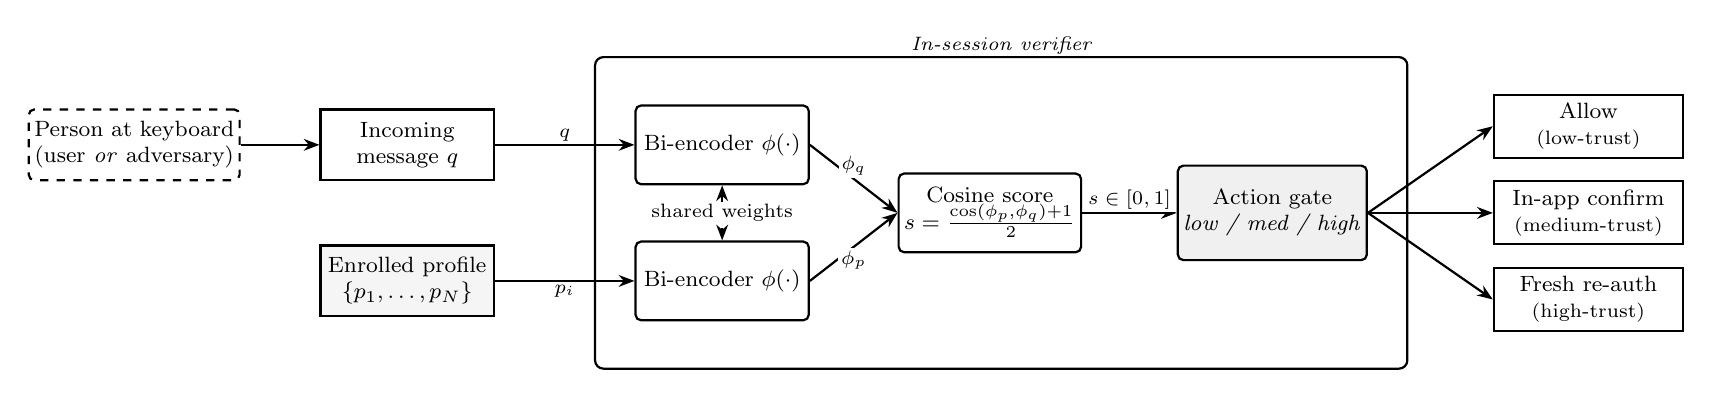
\begin{tikzpicture}[
    font=\footnotesize,
    >={Stealth[length=2mm]},
    block/.style={
        draw, thick, rounded corners=2pt,
        minimum width=22mm, minimum height=10mm,
        align=center, inner sep=2pt, fill=white
    },
    io/.style={
        draw, thick,
        minimum width=22mm, minimum height=9mm,
        align=center, inner sep=2pt, fill=white
    },
    profilebox/.style={
        draw, thick,
        minimum width=22mm, minimum height=9mm,
        align=center, inner sep=2pt, fill=gray!8
    },
    gate/.style={
        draw, thick, rounded corners=2pt,
        minimum width=22mm, minimum height=12mm,
        align=center, inner sep=2pt, fill=gray!12
    },
    actor/.style={
        draw, thick, dashed, rounded corners=2pt,
        minimum width=22mm, minimum height=9mm,
        align=center, inner sep=2pt
    },
    outcome/.style={
        draw, thick,
        minimum width=24mm, minimum height=8mm,
        align=center, inner sep=2pt, fill=white
    },
    arrow/.style={->, thick},
    midlabel/.style={font=\scriptsize, midway, fill=white, inner sep=1pt}
]

% --- Actor on the left ---
\node[actor] (typist) at (0,0) {Person at keyboard\\(user \emph{or} adversary)};

% --- Incoming message and stored profile ---
\node[io, right=10mm of typist] (msg) {Incoming\\message $q$};
\node[profilebox, below=8mm of msg] (profile) {Enrolled profile\\$\{p_1,\dots,p_N\}$};

% --- Shared bi-encoder: two instances of the SAME encoder (shared weights) ---
\node[block] (encq) at ($(msg) + (40mm,0)$)
    {Bi-encoder $\phi(\cdot)$};
\node[block] (encp) at ($(profile) + (40mm,0)$)
    {Bi-encoder $\phi(\cdot)$};
\draw[<->, thick, dashed] (encq.south) -- node[midlabel]{\scriptsize shared weights} (encp.north);

% --- Cosine score and action gate ---
\node[block] (score) at ($(encq)!0.5!(encp) + (34mm,0)$)
    {Cosine score\\$s=\tfrac{\cos(\phi_p,\phi_q)+1}{2}$};
\node[gate, right=12mm of score] (gateNode)
    {Action gate\\\textit{low / med / high}};

% --- Outcomes: wider gap so arrow labels do not overlap ---
\node[outcome] (allow)   at ($(gateNode.east) + (28mm, 11mm)$) {Allow\\\scriptsize(low-trust)};
\node[outcome] (confirm) at ($(gateNode.east) + (28mm,  0mm)$) {In-app confirm\\\scriptsize(medium-trust)};
\node[outcome] (block)   at ($(gateNode.east) + (28mm,-11mm)$) {Fresh re-auth\\\scriptsize(high-trust)};

% --- Typist to message ---
\draw[arrow] (typist.east) -- (msg.west);

% --- Message and profile each into their own copy of the shared encoder ---
\draw[arrow] (msg.east)     -- node[midlabel, above]{$q$}   (encq.west);
\draw[arrow] (profile.east) -- node[midlabel, below]{$p_i$} (encp.west);

% --- Each encoder output to cosine; cosine to gate ---
\draw[arrow] (encq.east) -- node[midlabel, above]{$\phi_q$} (score.west);
\draw[arrow] (encp.east) -- node[midlabel, below]{$\phi_p$} (score.west);
\draw[arrow] (score.east) -- node[midlabel, above]{$s\in[0,1]$}    (gateNode.west);

% --- Gate to outcomes (no on-arrow labels; tiers now inside outcome boxes) ---
\draw[arrow] (gateNode.east) -- (allow.west);
\draw[arrow] (gateNode.east) -- (confirm.west);
\draw[arrow] (gateNode.east) -- (block.west);

% --- Bounding box around verifier ---
\begin{scope}[on background layer]
    \node[
        fit=(encq)(encp)(score)(gateNode),
        draw, thick, rounded corners=3pt,
        inner xsep=5mm, inner ysep=6mm,
        label={[anchor=south, font=\scriptsize\itshape, yshift=-1mm]north:In-session verifier}
    ] (verifier) {};
\end{scope}

\end{tikzpicture}
}
\caption{System overview. A user interacts with an already-authenticated LLM agent session; the verifier has no prior knowledge of whether the active user is the legitimate account holder or an adversary. The in-session verifier (rounded box) encodes the enrolled profile $\{p_1,\dots,p_N\}$ and the incoming message $q$ \emph{independently} with the same shared-weight bi-encoder $\phi$ (there is no joint cross-encoder), scores their pooled cosine in $[0,1]$, and feeds the score to a tiered action gate (Section~\ref{sec:deployment}): low-trust actions are allowed silently, medium-trust actions require in-app confirmation when the score is below threshold, and high-trust actions require a fresh OS-level re-authentication.}
\label{fig:system_overview}
\end{figure*}

Figure~\ref{fig:system_overview} situates the verifier within an LLM agent session: an enrolled profile and an incoming message are encoded by a shared bi-encoder, their cosine score feeds a tiered action gate, and the gate's behaviour depends on the consequence class of the agent action being requested.

\noindent\textbf{The adversary.} We consider an adversary who has physical or session-level access to an LLM agent already enrolled for a legitimate user. The legitimate user has signed in at some point in the past, the agent may have access to the user's email, files, calendar, and MCP-connected tools, and the adversary is now using that same open session. The adversary's goal is to make the agent perform an action the legitimate user did not intend, such as sending a sensitive email, exfiltrating files, posting a message in the user's voice, or running a destructive shell command. The adversary types into the agent and can approve tool calls when the agent requests authorization. This adversary maps to OWASP LLM06 (Excessive Agency) and OWASP Agentic Applications ASI03 (Identity and Privilege Abuse), as discussed in Section~\ref{sec:intro}.

\noindent\textbf{What the adversary knows.} We give the adversary a realistic but nontrivial amount of knowledge. They may know the user's general topic distribution because they share a workplace, family, or social circle; they may know the projects, codebases, or clients the user works with; and they may attempt to mimic the user's writing style or register if they have seen the user write before. The adversary has access to neither the verifier's internal weights nor the enrolled profile stored on the device, which matches the on-device deployment setting we recommend later.

\noindent\textbf{What the defender sees.} The defender is the LLM agent. It holds an enrolled profile of the user's past messages and sees the new incoming text in the current session. The verifier produces a score and a decision using a fixed threshold selected on validation data, and does not get OS-level signals such as keystroke dynamics, mouse movement, or window focus; it only sees the text the user has typed. We treat the verifier as one layer in a defense-in-depth stack, not a replacement for OS-level authentication; the concrete policy mapping is in Section~\ref{sec:deployment}.

\noindent\textbf{Out of scope.} We do not study adversaries with direct access to the verifier weights, adversaries who have stolen the enrolled profile from the device (the on-device deployment assumption is already broken in that case), or adversaries who use another LLM to rewrite their messages in the user's style using examples of the user's writing.
\section{Related Work}

\noindent\textbf{Authorship verification.} Authorship verification has a long history in stylometry and the PAN evaluation campaigns have driven much of the modern work on it \citep{stamatatos2009survey,bevendorff2020overview}. The classical recipe combines character and word $n$-grams with shallow classifiers, and character $n$-grams in particular are known to mix style and topic signals in ways that can conflate style with topic/content signal \citep{sapkota2015notall}, which is one of the things we explicitly stress-test against in this paper. More recent work has moved to neural encoders: \citet{boenninghoff2019similarity} train hierarchical recurrent Siamese LSTM-based encoders for authorship verification on social media, \citet{barlas2020crossdomain} compare pre-trained language models against cross-domain authorship attribution, and \citet{tyo2022state} survey the broader state of the art across authorship and verification. Our contribution relative to this literature is twofold: we restructure PAN-20 from its native pairwise format into per-author profiles so that the task matches the deployment setting where an agent has an enrolled user history rather than two unrelated texts, and we stress-test the encoders against topic-similar imposters mined by an identity-agnostic similarity function instead of reporting only on the random or natural test distribution.

\noindent\textbf{Contrastive learning and hard-negative mining.} Siamese and bi-encoder objectives are standard in sentence representation learning, including triplet-network SBERT-style training \citep{reimers2019sentencebert} and contrastive sentence-embedding methods such as SimCSE \citep{gao2021simcse}; they also build on the broader metric-learning tradition exemplified by triplet loss in FaceNet \citep{schroff2015facenet}. Hard-negative mining is well studied in dense retrieval \citep{xiong2021ance} and in general contrastive and metric learning \citep{robinson2021hard,schroff2015facenet}, where easy random negatives can quickly become uninformative and semi-hard or hard negatives are often used to learn more discriminative representations. We apply the same idea to authorship verification specifically and evaluate the effect not just on threshold-free metrics like ROC-AUC but on the security operating points (TAR@FAR=1\%, FAR@FRR=1\%, catch@3 and median messages-to-detect) that a real agent deployment would care about, which is where most of the gains from hardness-aware training actually land.

\noindent\textbf{Concurrent work.} In concurrent work, \citet{shen2026chatbot} study dialogue attribution in unauthenticated human-LLM sessions, introducing WildAuth, a benchmark derived from real-world ChatGPT logs, and an uncertainty-aware multi-aspect attribution model. Our work and theirs are complementary but differ in three places: we frame the problem as an agent-layer security primitive with operating-point metrics (TAR@FAR=1\%, FAR@FRR=1\%, catch@3) rather than attribution accuracy alone; we add a hardness-stratified evaluation against topic-similar imposters so that the random-versus-hard robustness gap is observable; and we study a hardness-aware training regime alongside the random-trained baseline, which lets us measure whether the topic-vs-style shortcut is fixable through training rather than just diagnosed.

\section{Dataset}
\label{sec:dataset}

We use two complementary datasets. WildChat-1M \citep{zhao2024wildchat} is our primary dataset because it consists of real user-ChatGPT interactions and most closely approximates the agent-chat setting. PAN-20 \citep{bevendorff2020overview} is our secondary dataset because it is a widely used authorship-verification benchmark; using both allows us to test whether our findings hold across short conversational text and long fanfiction text.

\noindent\textbf{WildChat-1M.} We use the AllenAI release, filter to English-language users using the provided language field (mixing languages would let a verifier to exploit language ID rather than writing style), and use \texttt{hashed\_ip} as a proxy user identifier, following the dataset metadata. This is imperfect (shared-IP households merge identities, roaming users split them), which we discuss in the limitations. The model only ever sees raw user text. After filtering to English users with at least 10 messages, we obtain \textbf{16,467 eligible users}.

\noindent\textbf{PAN-20.} The official PAN-20 authorship-verification training release is in pairwise format, which does not match our deployment setting; we regroup it by author identifier across all pairs and treat each author as a single identity. After applying the same $\geq 10$-text filter we obtain \textbf{8,483 eligible authors}. PAN authors write fanfiction across multiple fandoms; we do not use fandom as a model input or a split key. PAN texts are much longer than WildChat messages (mean $\sim$21k characters), so we char-truncate at 2{,}000 before tokenization (defensive, not tuned).

\noindent\textbf{Preprocessing and counts.} We collapse repeated whitespace during model preprocessing but do not lowercase, strip punctuation, or remove special characters because punctuation habits and capitalization are exactly the stylometric signals the encoder should learn. After all filters, PAN gives a mean of 16.9 texts/author (11.4 profile, 5.5 query); WildChat gives 47.7 messages/user (33.0/14.7). The 60/20/20 author-disjoint split yields 5{,}090/1{,}697/1{,}696 on PAN and 9{,}880/3{,}294/3{,}293 on WildChat, identical across seeds (Table~\ref{tab:datastats}).

\begin{table}[t]
\centering
\small
\begin{tabular}{lrr}
\toprule
& \textbf{PAN-20} & \textbf{WildChat-1M} \\
\midrule
Eligible authors/users     & 8{,}483   & 16{,}467 \\
Mean texts per author      & 16.9      & 47.7 \\
\quad profile (70\%)       & 11.4      & 33.0 \\
\quad query (30\%)         & 5.5       & 14.7 \\
Mean chars/text            & $\sim$21k & $\sim$1.2k \\
Train / Val / Test         & 5090/1697/1696 & 9880/3294/3293 \\
\bottomrule
\end{tabular}
\caption{Dataset statistics after all filters. Train/val/test counts are identical across seeds 13, 21, 42 because the stratified shuffle preserves bucket sizes.}
\label{tab:datastats}
\end{table}

\section{Methodology}
\label{sec:method}


\noindent\textbf{Profile-query construction.} Each identity's text pool is split 70\%/30\% into profile (the enrolled history the agent has) and query (the new incoming text). For PAN we use a stable per-(seed, author) hash to shuffle and take the first 70\% as profile; for WildChat we sort messages chronologically by timestamp and take the first 70\% as profile and the last 30\% as query, matching the realistic deployment. We evaluate at two prefix lengths, $k{=}1$ (first held-out query message) and $k{=}3$ (first three averaged). Each author contributes one positive (profile vs.\ own query) and one negative (profile vs.\ another author's query) pair at every prefix length, so the evaluation set is balanced.

\noindent\textbf{Author-disjoint stratified splits.} We split authors 60/20/20 into train, validation and test with no overlap. The split is stratified by text count: PAN authors into 10--12, 13--16, 17--20, 21+ buckets; WildChat users into 10--12, 13--16, 17--20, 21--49, 50--99, 100--499, 500+. We deliberately do not split on topic or fandom: holding fandom shared but authors disjoint puts the verifier in the realistic situation (same topic, different writer), which is the only situation in which the random and hard test regimes have room to differ. The three seeds are 13, 21, 42; every reported number is the mean over them with sample standard deviation.

\noindent\textbf{Hardness mining.} A hard imposter is a different identity whose text looks similar to the anchor's under an identity-agnostic similarity function. For each identity $A$ in a split we rank every other identity $B$ by $\cos(\phi(\text{profile}_A), \phi(\text{query}_B))$. The top 5\% forms the hard bucket, ranks 5-30\% the semi-hard bucket, and the random bucket is sampled uniformly from other identities without similarity weighting. For each triplet we sample a negative identity from the requested bucket and then a uniformly random text from that identity's pool, rather than the single most similar text, which would concentrate gradients on a few identities. The \textit{primary miner} is a TF-IDF cosine model combining character 3-5-grams and word 1-2-grams ($\min\_df{=}1$, word features capped at 200k, char at 300k), trained separately within each split on that split's profile and query texts. The \textit{secondary miner} is \texttt{sentence-transformers/all-MiniLM-L6-v2} \citep{reimers2019sentencebert}, used as a fixed encoder with mean pooling and L2 normalization. Hardness indexes are cached per (dataset, seed, split).

\noindent\textbf{Primary miner, step by step.} Concretely, within each split the TF-IDF miner (1) fits a character 3-5-gram and word 1-2-gram TF-IDF vectorizer on that split's profile and query texts ($\min\_df{=}1$, word vocabulary capped at 200k features and character vocabulary at 300k); (2) L2-normalizes the resulting vectors; (3) for each anchor identity $A$, computes the cosine similarity between $A$'s profile vector and every other identity $B$'s query vector; and (4) ranks the other identities by this similarity, assigning the top 5\% to the hard bucket and ranks 5-30\% to the semi-hard bucket. The vectorizer is fit separately per split, so no text from another split informs a split's hardness ranking, and the resulting indexes are cached per (dataset, seed, split). The exact configuration and implementation are included in the released code.

\noindent\textbf{Contrastive bi-encoder and triplet loss.} A single transformer backbone with shared weights encodes the anchor, positive and negative texts independently. We load each encoder from \texttt{AutoModel} rather than \texttt{AutoModelForSequenceClassification}: the latter adds a task-specific classification head, whereas we need the encoder representation directly. For every text we mean-pool the last hidden state weighted by the attention mask and L2-normalize the pooled vector; we add no projection head, no custom special tokens and no prefix prompts, and use the stock tokenizer with $\text{max\_length}=256$. We train with triplet margin loss in Euclidean space with margin $0.3$. Because embeddings are L2-normalized, squared Euclidean distance is monotonic in cosine similarity ($\|a-b\|^2 = 2 - 2\cos(a,b)$), so the loss encourages anchor-positive cosine to exceed anchor-negative cosine, aligning training with the cosine-based evaluation score. We do not use in-batch negatives, which keeps the fraction of hard negatives a property of the sampler rather than the batch. Triplets are resampled every epoch with a per-epoch seed derived from the run seed.

\noindent\textbf{Two training regimes.} We compare two ways of choosing the training negatives: (i) \textbf{random-only}, with 100\% random negatives; and (ii) \textbf{mixed}, with 50\% random, 30\% semi-hard and 20\% hard negatives. The mixed proportions match the mixed test composition by design. The two regimes differ only in negative composition; everything else is held fixed, which lets us attribute any difference to the negative composition.

\noindent\textbf{Test protocol and scoring.} Each profile text is encoded independently, embeddings are averaged and re-L2-normalized to give one profile embedding per author, and the same is done for the query at each prefix length. The verification score is $(\cos+1)/2$, which is monotonic in cosine and preserves rank-based metrics. We score with fixed cosine rather than a learned pair scorer because cosine is symmetric, parameter-free, and generalizes to authors unseen during training, which matches our author-disjoint protocol; we discuss learned symmetric scorers as a future ablation in Section~\ref{sec:conclusion}. The decision threshold is selected once on mixed-regime validation predictions by maximising F1 and applied across all four test regimes: \textbf{random} (100\% random imposters), \textbf{semi-hard} (100\% from the 5-30\% bucket), \textbf{hard} (100\% from the top 5\% bucket), and \textbf{mixed} (50/30/20, the realistic deployment composition). The positives are identical across regimes, so any difference is attributable to imposter hardness. To check that our findings are not an artifact of the TF-IDF definition of ``hard'', we also run a secondary SBERT-miner ablation on DistilBERT and BERT in three configurations (random-only with SBERT test imposters; mixed TF-IDF train with SBERT test imposters; mixed SBERT on both sides).

\section{Experimental Setup}
\label{sec:expsetup}

\noindent\textbf{Models.} We evaluate four pre-trained transformer encoders in the TF-IDF hardness regime: DistilBERT-base-uncased \citep{sanh2019distilbert} (66M parameters), BERT-base-uncased \citep{devlin2019bert} (110M), MiniLM-L6 (\texttt{sentence-transformers/all-MiniLM-L6-v2}, 22.71M; an SBERT-pretrained MiniLM checkpoint \citep{reimers2019sentencebert}), and ELECTRA-base-discriminator \citep{clark2020electra} (110M). The four encoders span the compact-to-base size range that fits within our 8\,GB VRAM constraint. The SBERT cross-miner ablation is restricted to DistilBERT and BERT.

\noindent\textbf{Hyperparameters.} Triplets per identity per epoch are fixed at 16, giving 81{,}440 and 158{,}080 triplets per training epoch on PAN ($5{,}090 \times 16$) and WildChat ($9{,}880 \times 16$). Texts are char-truncated to 2{,}000 chars and tokenized at $\text{max\_length}=256$ with truncation. Train batch size is 16 for DistilBERT and MiniLM, and 8 with gradient accumulation 2 for BERT and ELECTRA (effective batch 16, fits within 8\,GB VRAM); eval batch size is 32 for DistilBERT/MiniLM and 16 for BERT/ELECTRA. Optimizer is AdamW with $\text{lr}=2\!\times\!10^{-5}$, weight decay 0.01, no warmup, gradient clipping at L2-norm 1.0, and FP16 mixed precision. We train for 3 epochs and select the best epoch by validation ROC-AUC, using the \textit{mixed} validation regime for both training regimes so that both pick their best checkpoint against the same difficulty distribution.

\noindent\textbf{Metrics.} We frame the task as a security problem, so alongside threshold-free summaries we report operating-point metrics. We treat genuine (same-author) pairs as the positive class throughout, so True Accept Rate (TAR) equals the true-positive rate (TPR) and False Accept Rate (FAR) equals the false-positive rate (FPR); the reverse convention, with imposters as positive, maps these to TNR and FNR. ROC-AUC (area under the receiver-operating-characteristic curve) summarizes ranking quality across all thresholds and is invariant to class balance; PR-AUC (area under the precision-recall curve) summarizes the precision-recall trade-off and, unlike ROC-AUC, depends on class prevalence. Because our evaluation set is balanced by construction (one genuine and one imposter pair per author), the two are numerically close here and we report both as complementary rank summaries; a deployment with its own genuine/imposter prevalence should recompute PR-AUC at that operating prevalence. \textbf{F1} is computed at the validation-selected threshold, held fixed across test regimes and prefix lengths. \textbf{EER} (Equal Error Rate) is the operating point where false-accept and false-reject rates meet. \textbf{TAR@FAR=1\%} answers ``if we are only willing to let 1 imposter in 100 slip through, what fraction of legitimate users do we accept?''; \textbf{FAR@FRR=1\%} answers the symmetric question (what fraction of imposters we accept when only 1 in 100 genuine users is rejected). For streaming detection over the first query messages we report \textbf{catch@3} (fraction of imposters whose averaged 3-message score falls below threshold), the genuine survival rate at 3 (fraction of genuine users still accepted after three messages), and \textbf{median messages-to-detect}: among imposters that are eventually caught, the median first prefix $k\in\{1,3\}$ at which the score falls below the fixed threshold. Because we evaluate only two prefix lengths, messages-to-detect is a coarse two-point measure (its value is $1$ or $3$); we therefore report it alongside catch@3 rather than on its own, and also report its P90.

\noindent\textbf{Hardware and reproducibility.} All contrastive experiments were run on a single workstation with an RTX 4060\,Ti (8\,GB VRAM), Intel i9-13900K, and 31\,GB RAM; we use FP16 mixed precision to fit BERT and ELECTRA. Each (dataset, model, regime, seed) contrastive cell takes 2-3 hours including evaluation on all four test regimes. We do not sweep hyperparameters: the per-model-class settings above are held fixed across all cells. We release the source code, preprocessing and split-generation scripts, configs, evaluation code, and result JSONs; raw text files are not redistributed because both datasets contain user-sensitive content, but splits can be reconstructed deterministically from the released seeds.

\section{Results}
\label{sec:results}

All aggregate numbers in the main tables are means over seeds 13, 21 and 42; sample standard deviations are reported in the appendix. Table~\ref{tab:main_hard} gives the headline Hard-regime results, Table~\ref{tab:robustness_gap} gives the random-to-hard robustness gap per encoder, and Table~\ref{tab:sbert_ablation} gives the SBERT cross-miner ablation on DistilBERT and BERT. The full per-test-regime breakdown for the contrastive and SBERT-ablation runs is in Appendix~\ref{sec:appendix_full}.

\begin{table*}[!t]
\centering
\scriptsize
\setlength{\tabcolsep}{3pt}
\begin{tabular}{l l r r @{\hspace{1.7em}} r r @{\hspace{1.7em}} r r @{\hspace{1.7em}} r r}
\toprule
& & \multicolumn{2}{c}{\textbf{ROC-AUC}} & \multicolumn{2}{c}{\textbf{TAR@FAR=1\%}} & \multicolumn{2}{c}{\textbf{catch@3}} & \multicolumn{2}{c}{\textbf{EER}} \\
\cmidrule(lr){3-4}\cmidrule(lr){5-6}\cmidrule(lr){7-8}\cmidrule(lr){9-10}
\textbf{Dataset} & \textbf{Encoder} & RO & Mix & RO & Mix & RO & Mix & RO & Mix \\
\midrule
\multicolumn{10}{l}{\textit{Reference baselines (no contrastive fine-tuning)}} \\
PAN-20  & TF-IDF cosine     & \multicolumn{2}{c}{95.4} & \multicolumn{2}{c}{82.3} & \multicolumn{2}{c}{81.4} & \multicolumn{2}{c}{11.0} \\
PAN-20  & SBERT-mpnet       & \multicolumn{2}{c}{68.8} & \multicolumn{2}{c}{16.4} & \multicolumn{2}{c}{\phantom{0}4.5} & \multicolumn{2}{c}{37.6} \\
PAN-20  & Frozen DistilBERT & \multicolumn{2}{c}{73.5} & \multicolumn{2}{c}{27.1} & \multicolumn{2}{c}{\phantom{0}5.9} & \multicolumn{2}{c}{36.2} \\
PAN-20  & Frozen BERT       & \multicolumn{2}{c}{73.3} & \multicolumn{2}{c}{29.7} & \multicolumn{2}{c}{\phantom{0}3.6} & \multicolumn{2}{c}{37.2} \\
PAN-20  & Frozen MiniLM     & \multicolumn{2}{c}{69.9} & \multicolumn{2}{c}{19.7} & \multicolumn{2}{c}{\phantom{0}4.4} & \multicolumn{2}{c}{37.4} \\
PAN-20  & Frozen ELECTRA    & \multicolumn{2}{c}{74.1} & \multicolumn{2}{c}{21.8} & \multicolumn{2}{c}{17.3} & \multicolumn{2}{c}{33.4} \\
WildChat & TF-IDF cosine     & \multicolumn{2}{c}{74.5} & \multicolumn{2}{c}{\phantom{0}1.4} & \multicolumn{2}{c}{54.4} & \multicolumn{2}{c}{28.2} \\
WildChat & SBERT-mpnet       & \multicolumn{2}{c}{81.9} & \multicolumn{2}{c}{\phantom{0}4.5} & \multicolumn{2}{c}{65.6} & \multicolumn{2}{c}{21.6} \\
WildChat & Frozen DistilBERT & \multicolumn{2}{c}{73.9} & \multicolumn{2}{c}{\phantom{0}3.4} & \multicolumn{2}{c}{41.9} & \multicolumn{2}{c}{30.1} \\
WildChat & Frozen BERT       & \multicolumn{2}{c}{72.8} & \multicolumn{2}{c}{\phantom{0}3.5} & \multicolumn{2}{c}{39.8} & \multicolumn{2}{c}{31.0} \\
WildChat & Frozen MiniLM     & \multicolumn{2}{c}{82.9} & \multicolumn{2}{c}{\phantom{0}5.7} & \multicolumn{2}{c}{67.7} & \multicolumn{2}{c}{20.7} \\
WildChat & Frozen ELECTRA    & \multicolumn{2}{c}{62.4} & \multicolumn{2}{c}{\phantom{0}3.2} & \multicolumn{2}{c}{18.5} & \multicolumn{2}{c}{40.4} \\
\midrule
\multicolumn{10}{l}{\textit{Contrastive fine-tuning}} \\
\multirow{4}{*}{PAN-20}
 & DistilBERT & 93.4 & \textbf{93.9} & 43.9 & \textbf{46.1} & 74.9 & \textbf{77.4} & 14.4 & \textbf{13.9} \\
 & BERT       & 94.2 & \textbf{94.5} & 48.8 & \textbf{50.9} & 76.7 & \textbf{79.1} & 13.3 & \textbf{13.2} \\
 & MiniLM     & 92.0 & \textbf{92.2} & 39.1 & \textbf{40.7} & 73.4 & \textbf{73.7} & 16.0 & 16.0 \\
 & ELECTRA    & 94.2 & \textbf{94.7} & 47.1 & \textbf{50.6} & 75.7 & \textbf{78.6} & 13.2 & \textbf{12.9} \\
\midrule
\multirow{4}{*}{WildChat}
 & DistilBERT & 86.7 & \textbf{89.6} & \phantom{0}7.3 & \textbf{20.3} & 65.2 & \textbf{69.1} & 19.9 & \textbf{18.3} \\
 & BERT       & 86.4 & \textbf{89.8} & \phantom{0}6.2 & \textbf{22.3} & 65.0 & \textbf{69.6} & 20.1 & \textbf{18.3} \\
 & MiniLM     & 89.0 & \textbf{90.6} & 21.7 & \textbf{23.7} & 67.5 & \textbf{69.8} & 18.8 & \textbf{17.4} \\
 & ELECTRA    & 85.1 & \textbf{87.6} & \phantom{0}4.3 & \phantom{0}\textbf{9.9} & 62.4 & \textbf{65.7} & 21.3 & \textbf{19.6} \\
\bottomrule
\end{tabular}
\caption{Main results on the \textbf{Hard} test regime (top 5\% similarity imposters), means over seeds 13/21/42 (\%). ROC-AUC, TAR@FAR=1\%, and EER are computed over pooled $k{=}1$ and $k{=}3$ predictions; catch@3 uses the $k{=}3$ prefix. Reference baselines (top block) are evaluated without contrastive fine-tuning; their single score per metric is shown under both RO and Mix columns via \texttt{\textbackslash multicolumn}. ``SBERT-mpnet'' uses \texttt{sentence-transformers/all-mpnet-base-v2}; ``Frozen MiniLM'' uses \texttt{sentence-transformers/all-MiniLM-L6-v2}, a sentence-similarity-pretrained checkpoint. RO = random-only training, Mix = 50/30/20 random/semi-hard/hard training. For each RO/Mix pair we \textbf{bold} the better value (higher for ROC-AUC, TAR@FAR=1\% and catch@3; lower for EER). Hardness-aware training delivers the largest gains on WildChat, particularly on TAR@FAR=1\%. See Appendix~\ref{sec:appendix_full} for the full per-regime breakdown with sample standard deviations.}
\label{tab:main_hard}
\end{table*}

\begin{center}
\small
\begin{tabular}{l l rrr}
\toprule
\textbf{Dataset} & \textbf{Encoder} & \textbf{RO} & \textbf{Mix} & \textbf{$\Delta$} \\
\midrule
\multirow{4}{*}{PAN-20}
 & DistilBERT & 3.42 & 2.58 & $-$0.84 \\
 & BERT       & 2.91 & 2.43 & $-$0.48 \\
 & MiniLM     & 3.61 & 2.81 & $-$0.80 \\
 & ELECTRA    & 2.92 & 2.15 & $-$0.76 \\
\midrule
\multirow{4}{*}{WildChat}
 & DistilBERT & 9.54 & 6.78 & $-$2.76 \\
 & BERT       & 9.85 & 6.51 & $-$3.33 \\
 & MiniLM     & 7.55 & 5.85 & $-$1.70 \\
 & ELECTRA    & 10.63 & 8.23 & $-$2.41 \\
\bottomrule
\end{tabular}
\captionof{table}{Random-to-Hard ROC-AUC \textbf{robustness gap} per encoder (\%, lower is better). $\Delta$ = Mix$-$RO; negative means the gap shrank under hardness-aware training. WildChat shows the largest reductions, consistent with WildChat having the largest random-only gap.}
\label{tab:robustness_gap}
\end{center}

\begin{center}
\small
\begin{tabular}{l l rr}
\toprule
 & & \multicolumn{2}{c}{\textbf{Hard regime}} \\
 \cmidrule(lr){3-4}
\textbf{Setting} & \textbf{Model} & ROC-AUC & TAR@FAR=1\% \\
\midrule
\multicolumn{4}{l}{\textit{TF-IDF eval (Mix orig)}} \\
PAN      & DistilBERT  & 94.0 & 46.1 \\
PAN      & BERT        & 94.5 & 50.9 \\
WildChat & DistilBERT  & 89.6 & 20.3 \\
WildChat & BERT        & 89.8 & 22.3 \\
\midrule
\multicolumn{4}{l}{\textit{SBERT eval, RO training}} \\
PAN      & DistilBERT  & 94.0 & 46.0 \\
PAN      & BERT        & 94.5 & 49.8 \\
WildChat & DistilBERT  & 83.5 & \phantom{0}7.4 \\
WildChat & BERT        & 83.1 & \phantom{0}5.2 \\
\midrule
\multicolumn{4}{l}{\textit{SBERT eval, TF-IDF Mix training (cross-miner)}} \\
PAN      & DistilBERT  & 93.6 & 45.4 \\
PAN      & BERT        & 94.3 & 47.9 \\
WildChat & DistilBERT  & 85.8 & 18.6 \\
WildChat & BERT        & 85.9 & 18.6 \\
\midrule
\multicolumn{4}{l}{\textit{SBERT eval, SBERT Mix training (same-miner)}} \\
PAN      & DistilBERT  & 94.4 & 48.5 \\
PAN      & BERT        & 94.8 & 49.7 \\
WildChat & DistilBERT  & 86.6 & 20.3 \\
WildChat & BERT        & 86.4 & 18.3 \\
\bottomrule
\end{tabular}
\captionof{table}{SBERT cross-miner ablation on DistilBERT and BERT, Hard regime only (\%). The topic-vs-style gap and the hardness-aware fix both replicate when the test imposters are mined by SBERT instead of TF-IDF, so the finding is not an artifact of the specific definition of ``hard''.}
\label{tab:sbert_ablation}
\end{center}

\noindent\textbf{Reference baselines.} The top block of Table~\ref{tab:main_hard} reports three training-free families. On PAN, TF-IDF cosine is surprisingly strong on Hard (ROC-AUC 95.4, TAR@FAR=1\% 82.3), outperforming every fine-tuned encoder; this matches prior observations that $n$-gram methods remain competitive on long, content-rich authorship tasks \citep{tyo2022state}. On WildChat (texts roughly 18$\times$ shorter), TF-IDF degrades sharply at the strict operating point (TAR@FAR=1\% 1.4), and the strongest training-free verifier is the frozen \texttt{all-MiniLM-L6-v2} checkpoint (ROC-AUC 82.9, TAR@FAR=1\% 5.7), which already benefits from sentence-similarity pretraining; SBERT-mpnet zero-shot is slightly below it. Frozen DistilBERT, BERT, and ELECTRA are weak on WildChat (TAR@FAR=1\% 3.2-3.5), so off-the-shelf transformer embeddings without sentence-level pretraining are poor zero-shot verifiers here. BERT and DistilBERT Mix (TAR@FAR=1\% 22.3 and 20.3) reach roughly 4$\times$ the best training-free WildChat number.

\noindent\textbf{The encoders look strong on random imposters but struggle on topic-similar ones.} Across all four encoders the random-imposter regime looks strong by ROC-AUC (0.95-0.97 on both datasets), though the stricter TAR@FAR=1\% metric is much lower on WildChat random (45-63\%). The hard regime is a different story. Under random-only training, ROC-AUC drops from 0.96-0.97 random to 0.85-0.89 hard on WildChat (9.85 points for BERT, 9.54 for DistilBERT, 10.63 for ELECTRA, 7.55 for MiniLM), and TAR@FAR=1\% on WildChat Hard collapses to 6.2\% (BERT), 7.3\% (DistilBERT), 4.3\% (ELECTRA) and 21.7\% (MiniLM). On PAN the drops are smaller (2.9-3.6 ROC-AUC points), consistent with PAN texts being long and content-rich enough that the encoder has more style signal to fall back on, but the gap is present on every encoder.

\noindent\textbf{Hardness-aware training substantially reduces the WildChat gap.} The 50/30/20 mix shrinks the WildChat random-to-hard ROC-AUC gap by 22-34\% across encoders (Table~\ref{tab:robustness_gap}); the PR-AUC gap roughly halves on BERT (13.84 $\to$ 7.56) and DistilBERT (12.88 $\to$ 7.91). The biggest absolute gain lands on TAR@FAR=1\% on WildChat Hard, the metric a security team would deploy on: 6.2\% $\to$ 22.3\% for BERT (+16.2 points) and 7.3\% $\to$ 20.3\% for DistilBERT (+12.9 points), with the corresponding WildChat Mixed-test TAR@FAR=1\% climbing 18.9\% $\to$ 42.2\% (BERT) and 22.3\% $\to$ 41.9\% (DistilBERT). PAN gains are smaller (+1.5 to +3.5 TAR@FAR=1\% on Hard), expected given the small PAN random-only gap. Hardness-aware training matters most where the gap is large.

\noindent\textbf{Streaming detection is fast when it fires.} On WildChat Hard, catch@3 reaches 69.6\% for BERT and 69.1\% for DistilBERT under mixed training, up from 65.0\% and 65.2\% under random-only training. The median messages-to-detect is one across all four encoders, both datasets, and all test regimes in the main contrastive runs, so in the cases where the verifier flags the imposter it usually does so on the first message. On the realistic WildChat mixed-test distribution, catch@3 sits at 85.1\% for BERT and 85.0\% for DistilBERT under mixed training.

\noindent\textbf{The SBERT cross-miner ablation reproduces the direction.} Swapping the test imposters from TF-IDF to SBERT-mined drops the WildChat Hard ROC-AUC by about 4 points for the TF-IDF-mixed model (BERT 89.76 $\rightarrow$ 85.95, DistilBERT 89.60 $\rightarrow$ 85.75). Training on SBERT-mined negatives gives a modest additional ROC-AUC gain (BERT 86.43, DistilBERT 86.60), while the larger effect is visible at the strict operating point. Under SBERT evaluation, WildChat Hard TAR@FAR=1\% rises from 5.2\% to 18.3\% for BERT and from 7.4\% to 20.3\% for DistilBERT, so the topic-vs-style gap and the hardness-aware fix are not artifacts of the TF-IDF definition of ``hard''. On PAN, the SBERT cross-miner numbers stay close to the TF-IDF numbers, consistent with PAN being a less hardness-sensitive dataset.

\section{Deployment Recommendations}
\label{sec:deployment}

The results in this paper indicate that the verifier is not strong enough to be a deployment's only line of defense, but it is useful as one layer when combined with the controls OWASP recommends for LLM06 \citep{owasp2025llm}. We translate the operating-point numbers into concrete agent-side policies that a deployment could implement without changing the underlying model.

\noindent\textbf{Action categories.} Following OWASP LLM06's emphasis on minimizing agency and requiring human approval for high-impact actions, we organize agent actions by consequence into three deployment tiers. \textit{Low-trust} actions are non-sensitive reads and short responses that do not change persistent state (answering a factual question, fetching a public URL), where a wrong verdict is recoverable in both directions. \textit{Medium-trust} actions change persistent state in visible and recoverable ways (drafting an email but not sending it, creating a calendar event, editing a file in the user's workspace, committing code that has not been pushed). \textit{High-trust} actions carry incident-level risk (sending email, transferring funds, running shell commands, modifying access tokens, posting publicly in the user's voice, or calling an MCP tool that changes an external system).

\noindent\textbf{Suggested policy.} For low-trust actions, the verifier is run silently and its score is logged for telemetry; no blocking is performed. For medium-trust actions, the verifier is used as a risk signal, with lightweight step-up confirmation required when the score falls below a threshold. For high-trust actions, the verifier is not sufficient on its own; fresh OS-level authentication (biometric, password, or hardware token), re-enrollment of the agent session, or a delay sufficient for session expiry and screen-lock mechanisms to trigger is required. The verifier's role at this tier is to flag the session and raise the friction the legitimate user has to clear, not to make the trust call by itself. Because the verifier scores every incoming message, a rolling three-message monitor can escalate the next medium-trust action to high-trust treatment if the score drops below threshold mid-session. At a strict 1\% false-accept budget on WildChat Hard, the verifier still rejects roughly 80\% of legitimate attempts, too friction-heavy to gate medium-trust actions on its own; adaptive thresholds, longer profiles, and behavioral biometrics are the natural levers.

\noindent\textbf{Profile updating and drift.} Our benchmark assumes a fixed enrolled profile and therefore does not specify a deployment refresh schedule. In practice, profiles may need periodic updates as writing style changes, but indiscriminately adding accepted messages is unsafe: a single false accept can gradually poison the enrolled representation. A safer policy would refresh cached profile embeddings only with messages that pass a high-confidence check or follow fresh OS-level re-authentication, while retaining a stable historical component and bounding the recent-message window; the globally trained bi-encoder weights remain fixed. We leave refresh frequency and poisoning-resistant update policies to future work. Online cost remains low: with profile embeddings cached at enrollment, each new message requires only one forward pass and one cosine comparison.

\section{Conclusion}
\label{sec:conclusion}

We study whether a text encoder can serve as an agent-layer identity check for LLM-driven desktop agents, using a profile–query authorship verification benchmark from WildChat-1M and a regrouped PAN-20. Fine-tuned contrastive bi-encoders look strong against random imposters (ROC-AUC above 0.95) but rely heavily on topic and vocabulary, so WildChat ROC-AUC drops 8--11 points and TAR@FAR=1\% collapses into the single digits once the imposter shares the user's topic. A 50/30/20 mix of random, semi-hard and hard imposters substantially reduces this gap, with the largest gains on TAR@FAR=1\% (WildChat Hard 6--7\% $\to$ 20--22\% for BERT and DistilBERT) and the direction holding under a secondary SBERT miner. The absolute numbers are still not strong enough for the verifier to be a deployment's only line of defense, so we recommend the tiered policy in Section~\ref{sec:deployment}.

We consider several follow-up points. First, a stronger adversary model where the imposter uses an LLM to actively rewrite messages in the user's style; our current imposters are real topic-similar users, not adversarial mimics. Second, longer enrollment profiles plus behavioral signals (keystroke timing, action patterns) to push TAR@FAR=1\% high enough for medium-trust gating. Third, scaling to larger encoders and multilingual settings beyond English. Fourth, per-user calibration or lightweight adaptation on top of the globally trained encoder, which may capture user-specific writing cues that a shared model misses. Fifth, replacing the fixed cosine score with a symmetric learned scorer over embedding pairs, for example over the features $[\,|a-b|;\,a\odot b\,]$, which could model richer interactions provided it preserves symmetry and does not learn corpus-specific pair shortcuts. We release the benchmark construction scripts and evaluation code so these can be reproduced from the same setup.

\section*{Limitations}

In order to identify users in WildChat we use the \texttt{hashed\_ip} field, but this is imperfect because it suffers from the shared IP problem and a single user moving between networks can contribute multiple identities. We accept these caveats since the dataset is large enough that we expect noise to dilute when aggregated at scale, but a real deployment environment would need a more reliable identity signal than IP addresses.

Our results do not say anything about multilingual authorship verification, the case where an imposter uses a different language than the user, or the case where the same author uses different languages while communicating with the LLM. In WildChat we filter the dataset to English-language users only so that the verifier does not win the task just by detecting language ID instead of writing style.

The hard imposters in our datasets are real authors or normal users and not humans with malicious intent. A real adversary trying to impersonate a user will probably do something similar by matching topics or vocabulary, but we do not test the stronger case where the adversary actively tries to replicate the user's style.

All experiments were run on a single 8\,GB GPU, which limits us to models under approximately 200M parameters at our sequence length. We evaluate on four encoders (DistilBERT, BERT-base, MiniLM-L6 and ELECTRA-base) and the SBERT cross-miner ablation is run on two of these. We cannot verify whether the robustness gap closes at scale given the hardware constraint.

WildChat was collected in the early days when LLMs were just being released and most conversations are about coding help or short drafting tasks. It does not contain the chats where users ask an LLM to perform operations via MCP servers with access to delete files, read emails or access personal accounts, so a real deployment threat model is sharper than what we directly study. Related to this, we do not study the risk scores of imposter messages to determine how dangerous an accepted imposter would be; that is planned for follow-up work.

These constraints mean our findings should be read within the evaluated setting (English-only text, non-adaptive topic-similar imposters, encoders below 200M parameters) and not assumed to transfer directly to multilingual users, style-mimicking adversaries, or substantially larger encoders.

\section*{Ethics Statement}

Authorship verification is a double-edged sword: the techniques we study to refuse imposter sessions inside LLM agents can also be used to link anonymous online writing back to real people with known writings, which would be disastrous for users like whistleblowers, journalists and activists who depend on the right of anonymous speech. We did not invent the underlying techniques, but we want to be explicit that any deployment of this verifier outside the LLM-agent setting should be scrutinized carefully.

Beyond this, we recommend that deployments run on a user's on-premises device and the enrolled profiles themselves should not be sent to a central server or stored online. Moving user profiles into a remote backend database, even for legitimate verification purposes, creates aggregated datasets of how individuals write, which can become a target for both insider misuse and external attacks. Keeping the verifier on the user's device with the profile is a comparatively safer default because the writing style stays with the user.

PAN-20 is distributed under a research license and WildChat-1M is distributed under the license terms listed with the AllenAI release; we follow the terms of the exact dataset artifact used. Both datasets may contain sensitive content related to users in their texts, so we do not redistribute the texts and do not release any model checkpoint fine-tuned on individual user data. During training or evaluation the model never sees metadata fields such as \texttt{hashed\_ip}, country or \texttt{conversation\_id}; it only sees the user texts.

When the verifier is deployed inside an LLM agent, the cost of being wrong by accepting an imposter and by rejecting a legitimate user is not the same: a false accept can let the imposter take a consequential action, while a false reject merely requires the legitimate user to re-authenticate. We therefore operate in a strict setting where the verifier keeps out imposters even at the cost of rejecting some legitimate users, and we treat the verifier as one layer on top of OS-level login and per-action approval, not a replacement for them.

% Bibliography
\bibliography{custom}

\clearpage
\appendix

% Make appendix tables compact enough to pack cleanly on shared pages.
\raggedbottom
\captionsetup[table]{skip=3pt}
\renewcommand{\arraystretch}{0.85}
\setlength{\tabcolsep}{3pt}
\setcounter{topnumber}{4}
\setcounter{bottomnumber}{2}
\setcounter{totalnumber}{6}
\renewcommand{\topfraction}{0.95}
\renewcommand{\bottomfraction}{0.85}
\renewcommand{\textfraction}{0.05}
\renewcommand{\floatpagefraction}{0.80}
\makeatletter
\setlength{\@fptop}{0pt}
\setlength{\@dblfptop}{0pt}
\setlength{\@fpbot}{0pt plus 1fil}
\setlength{\@dblfpbot}{0pt plus 1fil}
\makeatother

\section{Full Per-Encoder Results (TF-IDF training)}
\label{sec:appendix_full}

This appendix reports the main metrics broken down by dataset, encoder, test regime and training regime. All numbers are mean $\pm$ sample standard deviation over seeds 13, 21 and 42, in percent. RO = random-only training; Mix = 50/30/20 hardness-aware training. Tables~\ref{tab:app_pan_distilbert}--\ref{tab:app_pan_electra} cover PAN-20, and Tables~\ref{tab:app_wc_distilbert}--\ref{tab:app_wc_electra} cover WildChat-1M. The compact random$\to$hard robustness-gap summary is reported in Table~\ref{tab:robustness_gap} in the main paper.

\paragraph{How to read these tables.} Each table has four \emph{test} blocks: \emph{Random} (uniformly sampled imposters), \emph{Semi-hard} (imposters from the 5--30\% TF-IDF similarity bucket), \emph{Hard} (top 5\% TF-IDF similarity), and \emph{Mixed} (the 50/30/20 deployment composition). Positives are identical across the four regimes, so any change in a row is attributable to imposter difficulty rather than to the genuine-user distribution. The RO and Mix columns hold the test set and the encoder fixed and vary only the training negative composition; the $\Delta$ column is Mix $-$ RO. A negative $\Delta$ on EER, FAR@FRR1\% or on the robustness gap is an improvement; a positive $\Delta$ on ROC-AUC, PR-AUC, F1, TAR@FAR1\% or catch@3 is an improvement.

\begin{table*}[!t]
\centering
\scriptsize
\begin{minipage}[t]{0.48\textwidth}
\centering
\begin{tabular}{l l c c c}
\toprule
\textbf{Test} & \textbf{Metric} & \textbf{RO} & \textbf{Mix} & \textbf{$\Delta$} \\
\midrule
Random    & ROC-AUC    & 96.78$\pm$0.43 & 96.53$\pm$0.56 & $-$0.25 \\
Random    & PR-AUC     & 96.89$\pm$0.41 & 96.60$\pm$0.50 & $-$0.28 \\
Random    & F1         & 90.39$\pm$0.80 & 89.80$\pm$1.10 & $-$0.58 \\
Random    & EER        & \phantom{0}9.60$\pm$0.83 & 10.16$\pm$1.09 & $+$0.56 \\
Random    & FAR@FRR1\% & 40.85$\pm$3.82 & 39.87$\pm$5.93 & $-$0.98 \\
Random    & TAR@FAR1\% & 62.78$\pm$2.80 & 59.85$\pm$2.14 & $-$2.94 \\
Random    & catch@3    & 88.88$\pm$2.26 & 87.70$\pm$1.20 & $-$1.18 \\
\midrule
Semi-hard & ROC-AUC    & 95.47$\pm$0.24 & 95.54$\pm$0.41 & $+$0.07 \\
Semi-hard & PR-AUC     & 95.67$\pm$0.11 & 95.65$\pm$0.34 & $-$0.02 \\
Semi-hard & F1         & 88.39$\pm$0.28 & 88.49$\pm$0.61 & $+$0.10 \\
Semi-hard & EER        & 11.60$\pm$0.40 & 11.49$\pm$0.71 & $-$0.11 \\
Semi-hard & FAR@FRR1\% & 52.16$\pm$4.21 & 48.44$\pm$5.42 & $-$3.72 \\
Semi-hard & TAR@FAR1\% & 56.08$\pm$1.90 & 55.62$\pm$2.45 & $-$0.46 \\
Semi-hard & catch@3    & 83.37$\pm$1.47 & 84.55$\pm$2.71 & $+$1.18 \\
\midrule
Hard      & ROC-AUC    & 93.36$\pm$0.24 & 93.95$\pm$0.22 & $+$0.59 \\
Hard      & PR-AUC     & 93.60$\pm$0.19 & 94.14$\pm$0.12 & $+$0.54 \\
Hard      & F1         & 85.39$\pm$0.37 & 86.33$\pm$0.33 & $+$0.94 \\
Hard      & EER        & 14.43$\pm$0.24 & 13.87$\pm$0.30 & $-$0.56 \\
Hard      & FAR@FRR1\% & 62.72$\pm$3.06 & 56.99$\pm$4.35 & $-$5.73 \\
Hard      & TAR@FAR1\% & 43.87$\pm$1.10 & 46.08$\pm$3.27 & $+$2.21 \\
Hard      & catch@3    & 74.94$\pm$1.68 & 77.44$\pm$1.47 & $+$2.50 \\
\midrule
Mixed     & ROC-AUC    & 95.67$\pm$0.44 & 95.65$\pm$0.69 & $-$0.02 \\
Mixed     & PR-AUC     & 95.85$\pm$0.43 & 95.77$\pm$0.68 & $-$0.08 \\
Mixed     & F1         & 88.64$\pm$0.47 & 88.75$\pm$0.75 & $+$0.12 \\
Mixed     & EER        & 11.47$\pm$0.54 & 11.40$\pm$0.93 & $-$0.07 \\
Mixed     & FAR@FRR1\% & 49.38$\pm$4.46 & 46.08$\pm$6.21 & $-$3.30 \\
Mixed     & TAR@FAR1\% & 55.67$\pm$3.11 & 55.40$\pm$5.19 & $-$0.27 \\
Mixed     & catch@3    & 84.00$\pm$1.81 & 84.67$\pm$1.78 & $+$0.67 \\
\bottomrule
\end{tabular}
\captionof{table}{PAN-20, DistilBERT-base-uncased (66M).}
\label{tab:app_pan_distilbert}
\end{minipage}%
\hfill
\begin{minipage}[t]{0.48\textwidth}
\centering
\begin{tabular}{l l c c c}
\toprule
\textbf{Test} & \textbf{Metric} & \textbf{RO} & \textbf{Mix} & \textbf{$\Delta$} \\
\midrule
Random    & ROC-AUC    & 97.10$\pm$0.39 & 96.97$\pm$0.24 & $-$0.13 \\
Random    & PR-AUC     & 97.22$\pm$0.34 & 97.03$\pm$0.25 & $-$0.19 \\
Random    & F1         & 91.02$\pm$0.74 & 90.56$\pm$0.63 & $-$0.46 \\
Random    & EER        & \phantom{0}9.00$\pm$0.74 & \phantom{0}9.34$\pm$0.42 & $+$0.33 \\
Random    & FAR@FRR1\% & 38.77$\pm$4.49 & 34.94$\pm$2.80 & $-$3.82 \\
Random    & TAR@FAR1\% & 63.74$\pm$2.35 & 62.15$\pm$4.60 & $-$1.59 \\
Random    & catch@3    & 89.39$\pm$2.55 & 89.64$\pm$1.05 & $+$0.26 \\
\midrule
Semi-hard & ROC-AUC    & 95.99$\pm$0.36 & 96.17$\pm$0.57 & $+$0.18 \\
Semi-hard & PR-AUC     & 96.18$\pm$0.25 & 96.33$\pm$0.54 & $+$0.14 \\
Semi-hard & F1         & 89.09$\pm$0.65 & 89.28$\pm$1.03 & $+$0.19 \\
Semi-hard & EER        & 10.90$\pm$0.58 & 10.71$\pm$1.01 & $-$0.19 \\
Semi-hard & FAR@FRR1\% & 48.44$\pm$4.93 & 42.75$\pm$3.88 & $-$5.69 \\
Semi-hard & TAR@FAR1\% & 59.22$\pm$1.97 & 61.17$\pm$3.56 & $+$1.96 \\
Semi-hard & catch@3    & 84.14$\pm$1.99 & 86.50$\pm$0.48 & $+$2.36 \\
\midrule
Hard      & ROC-AUC    & 94.18$\pm$0.39 & 94.54$\pm$0.43 & $+$0.35 \\
Hard      & PR-AUC     & 94.38$\pm$0.49 & 94.69$\pm$0.50 & $+$0.30 \\
Hard      & F1         & 86.47$\pm$0.47 & 86.96$\pm$0.53 & $+$0.49 \\
Hard      & EER        & 13.35$\pm$0.57 & 13.17$\pm$0.45 & $-$0.18 \\
Hard      & FAR@FRR1\% & 58.79$\pm$2.87 & 52.34$\pm$2.63 & $-$6.45 \\
Hard      & TAR@FAR1\% & 48.78$\pm$3.44 & 50.87$\pm$4.93 & $+$2.09 \\
Hard      & catch@3    & 76.67$\pm$1.66 & 79.07$\pm$1.84 & $+$2.40 \\
\midrule
Mixed     & ROC-AUC    & 96.10$\pm$0.46 & 96.00$\pm$0.64 & $-$0.10 \\
Mixed     & PR-AUC     & 96.26$\pm$0.44 & 96.06$\pm$0.64 & $-$0.20 \\
Mixed     & F1         & 89.25$\pm$0.83 & 89.16$\pm$1.17 & $-$0.09 \\
Mixed     & EER        & 10.82$\pm$0.78 & 10.94$\pm$1.00 & $+$0.12 \\
Mixed     & FAR@FRR1\% & 46.06$\pm$4.79 & 41.32$\pm$3.29 & $-$4.74 \\
Mixed     & TAR@FAR1\% & 59.06$\pm$2.88 & 56.49$\pm$3.68 & $-$2.57 \\
Mixed     & catch@3    & 84.65$\pm$1.92 & 85.61$\pm$0.81 & $+$0.96 \\
\bottomrule
\end{tabular}
\captionof{table}{PAN-20, BERT-base-uncased (110M).}
\label{tab:app_pan_bert}
\end{minipage}

\vspace{0.6em}

\begin{minipage}[t]{0.48\textwidth}
\centering
\begin{tabular}{l l c c c}
\toprule
\textbf{Test} & \textbf{Metric} & \textbf{RO} & \textbf{Mix} & \textbf{$\Delta$} \\
\midrule
Random    & ROC-AUC    & 95.64$\pm$0.60 & 95.03$\pm$0.44 & $-$0.60 \\
Random    & PR-AUC     & 95.77$\pm$0.58 & 95.16$\pm$0.45 & $-$0.60 \\
Random    & F1         & 88.75$\pm$1.00 & 87.74$\pm$0.50 & $-$1.02 \\
Random    & EER        & 11.22$\pm$1.01 & 12.34$\pm$0.67 & $+$1.12 \\
Random    & FAR@FRR1\% & 46.31$\pm$5.22 & 50.59$\pm$2.50 & $+$4.27 \\
Random    & TAR@FAR1\% & 53.98$\pm$3.60 & 51.40$\pm$1.53 & $-$2.58 \\
Random    & catch@3    & 86.79$\pm$1.56 & 84.00$\pm$1.10 & $-$2.79 \\
\midrule
Semi-hard & ROC-AUC    & 94.17$\pm$0.58 & 94.09$\pm$0.26 & $-$0.08 \\
Semi-hard & PR-AUC     & 94.41$\pm$0.37 & 94.32$\pm$0.17 & $-$0.09 \\
Semi-hard & F1         & 86.77$\pm$0.81 & 86.57$\pm$0.50 & $-$0.19 \\
Semi-hard & EER        & 13.26$\pm$0.86 & 13.71$\pm$0.53 & $+$0.45 \\
Semi-hard & FAR@FRR1\% & 55.90$\pm$6.78 & 56.72$\pm$1.85 & $+$0.83 \\
Semi-hard & TAR@FAR1\% & 48.48$\pm$1.81 & 48.87$\pm$0.61 & $+$0.39 \\
Semi-hard & catch@3    & 81.53$\pm$0.48 & 81.03$\pm$1.07 & $-$0.49 \\
\midrule
Hard      & ROC-AUC    & 92.03$\pm$0.60 & 92.22$\pm$0.26 & $+$0.20 \\
Hard      & PR-AUC     & 92.30$\pm$0.65 & 92.52$\pm$0.36 & $+$0.23 \\
Hard      & F1         & 84.18$\pm$0.61 & 84.31$\pm$0.24 & $+$0.13 \\
Hard      & EER        & 15.97$\pm$0.71 & 16.03$\pm$0.19 & $+$0.06 \\
Hard      & FAR@FRR1\% & 65.70$\pm$4.41 & 65.35$\pm$0.21 & $-$0.35 \\
Hard      & TAR@FAR1\% & 39.14$\pm$2.01 & 40.66$\pm$3.45 & $+$1.52 \\
Hard      & catch@3    & 73.45$\pm$0.70 & 73.74$\pm$0.53 & $+$0.29 \\
\midrule
Mixed     & ROC-AUC    & 94.39$\pm$0.89 & 94.14$\pm$0.54 & $-$0.25 \\
Mixed     & PR-AUC     & 94.56$\pm$0.87 & 94.30$\pm$0.52 & $-$0.26 \\
Mixed     & F1         & 87.05$\pm$1.10 & 86.85$\pm$1.01 & $-$0.20 \\
Mixed     & EER        & 13.01$\pm$1.20 & 13.35$\pm$0.91 & $+$0.33 \\
Mixed     & FAR@FRR1\% & 53.39$\pm$7.06 & 56.08$\pm$1.62 & $+$2.69 \\
Mixed     & TAR@FAR1\% & 48.09$\pm$6.58 & 47.40$\pm$2.07 & $-$0.70 \\
Mixed     & catch@3    & 82.04$\pm$1.62 & 81.27$\pm$2.08 & $-$0.77 \\
\bottomrule
\end{tabular}
\captionof{table}{PAN-20, MiniLM-L6 (22.71M).}
\label{tab:app_pan_minilm}
\end{minipage}%
\hfill
\begin{minipage}[t]{0.48\textwidth}
\centering
\begin{tabular}{l l c c c}
\toprule
\textbf{Test} & \textbf{Metric} & \textbf{RO} & \textbf{Mix} & \textbf{$\Delta$} \\
\midrule
Random    & ROC-AUC    & 97.10$\pm$0.13 & 96.85$\pm$0.57 & $-$0.25 \\
Random    & PR-AUC     & 97.19$\pm$0.16 & 96.96$\pm$0.49 & $-$0.22 \\
Random    & F1         & 91.06$\pm$0.18 & 90.60$\pm$1.06 & $-$0.46 \\
Random    & EER        & \phantom{0}8.95$\pm$0.09 & \phantom{0}9.49$\pm$0.94 & $+$0.54 \\
Random    & FAR@FRR1\% & 36.01$\pm$4.06 & 38.91$\pm$7.86 & $+$2.90 \\
Random    & TAR@FAR1\% & 63.37$\pm$1.99 & 62.73$\pm$3.91 & $-$0.65 \\
Random    & catch@3    & 88.74$\pm$1.20 & 88.09$\pm$0.93 & $-$0.65 \\
\midrule
Semi-hard & ROC-AUC    & 96.03$\pm$0.10 & 95.95$\pm$0.75 & $-$0.08 \\
Semi-hard & PR-AUC     & 96.25$\pm$0.19 & 96.12$\pm$0.65 & $-$0.13 \\
Semi-hard & F1         & 89.16$\pm$0.12 & 88.98$\pm$1.06 & $-$0.18 \\
Semi-hard & EER        & 10.59$\pm$0.10 & 11.03$\pm$1.18 & $+$0.43 \\
Semi-hard & FAR@FRR1\% & 45.57$\pm$5.01 & 45.74$\pm$7.44 & $+$0.18 \\
Semi-hard & TAR@FAR1\% & 58.91$\pm$2.88 & 58.24$\pm$3.87 & $-$0.68 \\
Semi-hard & catch@3    & 83.37$\pm$1.84 & 83.71$\pm$1.15 & $+$0.33 \\
\midrule
Hard      & ROC-AUC    & 94.18$\pm$0.33 & 94.70$\pm$0.59 & $+$0.52 \\
Hard      & PR-AUC     & 94.36$\pm$0.40 & 94.84$\pm$0.59 & $+$0.49 \\
Hard      & F1         & 86.56$\pm$0.19 & 87.26$\pm$0.55 & $+$0.70 \\
Hard      & EER        & 13.24$\pm$0.61 & 12.88$\pm$0.75 & $-$0.35 \\
Hard      & FAR@FRR1\% & 54.83$\pm$3.47 & 53.16$\pm$6.55 & $-$1.66 \\
Hard      & TAR@FAR1\% & 47.07$\pm$2.39 & 50.58$\pm$2.05 & $+$3.51 \\
Hard      & catch@3    & 75.69$\pm$1.76 & 78.62$\pm$1.89 & $+$2.93 \\
\midrule
Mixed     & ROC-AUC    & 96.02$\pm$0.32 & 95.91$\pm$0.85 & $-$0.10 \\
Mixed     & PR-AUC     & 96.09$\pm$0.34 & 96.05$\pm$0.79 & $-$0.04 \\
Mixed     & F1         & 89.22$\pm$0.29 & 88.94$\pm$1.38 & $-$0.27 \\
Mixed     & EER        & 10.83$\pm$0.33 & 11.01$\pm$1.44 & $+$0.18 \\
Mixed     & FAR@FRR1\% & 43.24$\pm$5.29 & 44.08$\pm$7.74 & $+$0.85 \\
Mixed     & TAR@FAR1\% & 54.50$\pm$2.02 & 57.11$\pm$3.21 & $+$2.61 \\
Mixed     & catch@3    & 83.61$\pm$0.89 & 83.67$\pm$1.37 & $+$0.06 \\
\bottomrule
\end{tabular}
\captionof{table}{PAN-20, ELECTRA-base-discriminator (110M).}
\label{tab:app_pan_electra}
\end{minipage}
\end{table*}

\begin{table*}[!t]
\centering
\scriptsize
\begin{minipage}[t]{0.48\textwidth}
\centering
\begin{tabular}{l l c c c}
\toprule
\textbf{Test} & \textbf{Metric} & \textbf{RO} & \textbf{Mix} & \textbf{$\Delta$} \\
\midrule
Random    & ROC-AUC    & 96.28$\pm$0.22 & 96.38$\pm$0.12 & $+$0.10 \\
Random    & PR-AUC     & 96.05$\pm$0.33 & 96.45$\pm$0.15 & $+$0.40 \\
Random    & F1         & 90.24$\pm$0.18 & 89.94$\pm$0.22 & $-$0.30 \\
Random    & EER        & \phantom{0}9.80$\pm$0.16 & 10.07$\pm$0.24 & $+$0.27 \\
Random    & FAR@FRR1\% & 43.88$\pm$1.57 & 44.94$\pm$1.19 & $+$1.06 \\
Random    & TAR@FAR1\% & 54.47$\pm$6.56 & 59.31$\pm$1.26 & $+$4.84 \\
Random    & catch@3    & 88.62$\pm$1.54 & 88.82$\pm$0.82 & $+$0.20 \\
\midrule
Semi-hard & ROC-AUC    & 95.05$\pm$0.27 & 95.60$\pm$0.24 & $+$0.55 \\
Semi-hard & PR-AUC     & 94.53$\pm$0.38 & 95.57$\pm$0.36 & $+$1.05 \\
Semi-hard & F1         & 88.74$\pm$0.28 & 89.07$\pm$0.25 & $+$0.33 \\
Semi-hard & EER        & 11.34$\pm$0.39 & 11.04$\pm$0.28 & $-$0.30 \\
Semi-hard & FAR@FRR1\% & 50.70$\pm$0.75 & 48.25$\pm$1.14 & $-$2.45 \\
Semi-hard & TAR@FAR1\% & 41.26$\pm$5.08 & 50.18$\pm$4.65 & $+$8.92 \\
Semi-hard & catch@3    & 85.06$\pm$2.32 & 86.88$\pm$0.90 & $+$1.82 \\
\midrule
Hard      & ROC-AUC    & 86.74$\pm$1.02 & 89.60$\pm$0.85 & $+$2.86 \\
Hard      & PR-AUC     & 83.17$\pm$1.37 & 88.54$\pm$1.26 & $+$5.37 \\
Hard      & F1         & 81.40$\pm$0.66 & 82.38$\pm$0.19 & $+$0.98 \\
Hard      & EER        & 19.89$\pm$0.92 & 18.26$\pm$0.89 & $-$1.63 \\
Hard      & FAR@FRR1\% & 73.89$\pm$0.41 & 69.37$\pm$1.21 & $-$4.52 \\
Hard      & TAR@FAR1\% & \phantom{0}7.31$\pm$0.95 & 20.25$\pm$6.91 & $+$12.94 \\
Hard      & catch@3    & 65.21$\pm$2.99 & 69.13$\pm$1.58 & $+$3.92 \\
\midrule
Mixed     & ROC-AUC    & 94.14$\pm$0.33 & 94.89$\pm$0.23 & $+$0.74 \\
Mixed     & PR-AUC     & 92.86$\pm$0.54 & 94.58$\pm$0.38 & $+$1.72 \\
Mixed     & F1         & 88.15$\pm$0.22 & 88.28$\pm$0.09 & $+$0.13 \\
Mixed     & EER        & 12.09$\pm$0.35 & 12.01$\pm$0.18 & $-$0.08 \\
Mixed     & FAR@FRR1\% & 51.20$\pm$0.36 & 49.94$\pm$1.23 & $-$1.26 \\
Mixed     & TAR@FAR1\% & 22.28$\pm$3.31 & 41.85$\pm$2.90 & $+$19.57 \\
Mixed     & catch@3    & 83.59$\pm$1.94 & 84.96$\pm$1.39 & $+$1.37 \\
\bottomrule
\end{tabular}
\captionof{table}{WildChat-1M, DistilBERT-base-uncased (66M).}
\label{tab:app_wc_distilbert}
\end{minipage}%
\hfill
\begin{minipage}[t]{0.48\textwidth}
\centering
\begin{tabular}{l l c c c}
\toprule
\textbf{Test} & \textbf{Metric} & \textbf{RO} & \textbf{Mix} & \textbf{$\Delta$} \\
\midrule
Random    & ROC-AUC    & 96.25$\pm$0.21 & 96.28$\pm$0.13 & $+$0.03 \\
Random    & PR-AUC     & 95.97$\pm$0.36 & 96.33$\pm$0.17 & $+$0.37 \\
Random    & F1         & 90.12$\pm$0.47 & 89.78$\pm$0.26 & $-$0.34 \\
Random    & EER        & \phantom{0}9.90$\pm$0.41 & 10.16$\pm$0.22 & $+$0.26 \\
Random    & FAR@FRR1\% & 42.78$\pm$0.98 & 43.06$\pm$1.74 & $+$0.28 \\
Random    & TAR@FAR1\% & 50.63$\pm$3.76 & 59.02$\pm$0.29 & $+$8.39 \\
Random    & catch@3    & 88.61$\pm$0.18 & 88.87$\pm$1.75 & $+$0.25 \\
\midrule
Semi-hard & ROC-AUC    & 94.97$\pm$0.28 & 95.54$\pm$0.25 & $+$0.56 \\
Semi-hard & PR-AUC     & 94.31$\pm$0.48 & 95.48$\pm$0.30 & $+$1.17 \\
Semi-hard & F1         & 88.66$\pm$0.42 & 88.86$\pm$0.52 & $+$0.20 \\
Semi-hard & EER        & 11.44$\pm$0.36 & 11.25$\pm$0.54 & $-$0.19 \\
Semi-hard & FAR@FRR1\% & 49.45$\pm$0.91 & 45.41$\pm$2.20 & $-$4.03 \\
Semi-hard & TAR@FAR1\% & 36.94$\pm$4.33 & 49.37$\pm$1.61 & $+$12.43 \\
Semi-hard & catch@3    & 84.97$\pm$0.20 & 86.57$\pm$1.77 & $+$1.60 \\
\midrule
Hard      & ROC-AUC    & 86.40$\pm$0.72 & 89.76$\pm$0.91 & $+$3.36 \\
Hard      & PR-AUC     & 82.13$\pm$1.14 & 88.78$\pm$1.26 & $+$6.65 \\
Hard      & F1         & 81.26$\pm$0.57 & 82.51$\pm$0.44 & $+$1.25 \\
Hard      & EER        & 20.11$\pm$0.65 & 18.28$\pm$0.94 & $-$1.83 \\
Hard      & FAR@FRR1\% & 72.59$\pm$0.64 & 66.36$\pm$1.63 & $-$6.24 \\
Hard      & TAR@FAR1\% & \phantom{0}6.17$\pm$0.55 & 22.32$\pm$3.94 & $+$16.15 \\
Hard      & catch@3    & 65.04$\pm$1.14 & 69.62$\pm$2.56 & $+$4.59 \\
\midrule
Mixed     & ROC-AUC    & 94.02$\pm$0.22 & 94.90$\pm$0.12 & $+$0.88 \\
Mixed     & PR-AUC     & 92.48$\pm$0.34 & 94.58$\pm$0.33 & $+$2.11 \\
Mixed     & F1         & 87.94$\pm$0.30 & 88.20$\pm$0.23 & $+$0.25 \\
Mixed     & EER        & 12.32$\pm$0.28 & 12.04$\pm$0.27 & $-$0.28 \\
Mixed     & FAR@FRR1\% & 50.27$\pm$0.64 & 47.77$\pm$2.38 & $-$2.50 \\
Mixed     & TAR@FAR1\% & 18.90$\pm$1.75 & 42.16$\pm$3.68 & $+$23.26 \\
Mixed     & catch@3    & 83.31$\pm$0.67 & 85.09$\pm$1.95 & $+$1.78 \\
\bottomrule
\end{tabular}
\captionof{table}{WildChat-1M, BERT-base-uncased (110M).}
\label{tab:app_wc_bert}
\end{minipage}

\vspace{0.6em}

\begin{minipage}[t]{0.48\textwidth}
\centering
\begin{tabular}{l l c c c}
\toprule
\textbf{Test} & \textbf{Metric} & \textbf{RO} & \textbf{Mix} & \textbf{$\Delta$} \\
\midrule
Random    & ROC-AUC    & 96.52$\pm$0.18 & 96.41$\pm$0.05 & $-$0.12 \\
Random    & PR-AUC     & 96.63$\pm$0.22 & 96.53$\pm$0.07 & $-$0.11 \\
Random    & F1         & 90.29$\pm$0.28 & 89.84$\pm$0.12 & $-$0.45 \\
Random    & EER        & \phantom{0}9.62$\pm$0.20 & 10.07$\pm$0.04 & $+$0.45 \\
Random    & FAR@FRR1\% & 47.49$\pm$1.39 & 44.24$\pm$1.15 & $-$3.26 \\
Random    & TAR@FAR1\% & 62.86$\pm$1.50 & 60.36$\pm$0.52 & $-$2.50 \\
Random    & catch@3    & 89.80$\pm$0.29 & 88.79$\pm$1.43 & $-$1.00 \\
\midrule
Semi-hard & ROC-AUC    & 95.58$\pm$0.16 & 95.86$\pm$0.03 & $+$0.28 \\
Semi-hard & PR-AUC     & 95.72$\pm$0.23 & 95.96$\pm$0.05 & $+$0.24 \\
Semi-hard & F1         & 89.09$\pm$0.28 & 89.16$\pm$0.19 & $+$0.06 \\
Semi-hard & EER        & 10.89$\pm$0.38 & 10.81$\pm$0.15 & $-$0.08 \\
Semi-hard & FAR@FRR1\% & 54.47$\pm$2.15 & 46.42$\pm$1.93 & $-$8.05 \\
Semi-hard & TAR@FAR1\% & 54.04$\pm$2.91 & 54.53$\pm$1.94 & $+$0.49 \\
Semi-hard & catch@3    & 86.73$\pm$0.44 & 87.06$\pm$1.29 & $+$0.33 \\
\midrule
Hard      & ROC-AUC    & 88.98$\pm$0.62 & 90.56$\pm$0.32 & $+$1.58 \\
Hard      & PR-AUC     & 88.17$\pm$0.71 & 89.91$\pm$0.66 & $+$1.74 \\
Hard      & F1         & 81.86$\pm$0.50 & 82.71$\pm$0.40 & $+$0.84 \\
Hard      & EER        & 18.83$\pm$0.89 & 17.37$\pm$0.36 & $-$1.47 \\
Hard      & FAR@FRR1\% & 76.80$\pm$2.01 & 67.62$\pm$1.85 & $-$9.19 \\
Hard      & TAR@FAR1\% & 21.67$\pm$2.14 & 23.75$\pm$6.48 & $+$2.08 \\
Hard      & catch@3    & 67.52$\pm$0.80 & 69.84$\pm$2.60 & $+$2.32 \\
\midrule
Mixed     & ROC-AUC    & 94.80$\pm$0.28 & 95.16$\pm$0.17 & $+$0.36 \\
Mixed     & PR-AUC     & 94.61$\pm$0.46 & 95.00$\pm$0.32 & $+$0.38 \\
Mixed     & F1         & 88.36$\pm$0.29 & 88.41$\pm$0.17 & $+$0.05 \\
Mixed     & EER        & 11.81$\pm$0.28 & 11.74$\pm$0.34 & $-$0.07 \\
Mixed     & FAR@FRR1\% & 54.98$\pm$1.88 & 48.80$\pm$0.29 & $-$6.17 \\
Mixed     & TAR@FAR1\% & 44.40$\pm$4.21 & 46.77$\pm$1.12 & $+$2.36 \\
Mixed     & catch@3    & 85.30$\pm$0.38 & 85.35$\pm$2.06 & $+$0.05 \\
\bottomrule
\end{tabular}
\captionof{table}{WildChat-1M, MiniLM-L6 (22.71M).}
\label{tab:app_wc_minilm}
\end{minipage}%
\hfill
\begin{minipage}[t]{0.48\textwidth}
\centering
\begin{tabular}{l l c c c}
\toprule
\textbf{Test} & \textbf{Metric} & \textbf{RO} & \textbf{Mix} & \textbf{$\Delta$} \\
\midrule
Random    & ROC-AUC    & 95.71$\pm$0.47 & 95.79$\pm$0.32 & $+$0.09 \\
Random    & PR-AUC     & 95.23$\pm$0.69 & 95.65$\pm$0.45 & $+$0.43 \\
Random    & F1         & 89.38$\pm$0.71 & 89.28$\pm$0.40 & $-$0.10 \\
Random    & EER        & 10.76$\pm$0.66 & 10.73$\pm$0.37 & $-$0.02 \\
Random    & FAR@FRR1\% & 44.62$\pm$3.01 & 47.90$\pm$1.06 & $+$3.28 \\
Random    & TAR@FAR1\% & 45.23$\pm$6.05 & 52.85$\pm$4.46 & $+$7.62 \\
Random    & catch@3    & 86.89$\pm$1.01 & 87.05$\pm$1.32 & $+$0.16 \\
\midrule
Semi-hard & ROC-AUC    & 94.36$\pm$0.37 & 94.80$\pm$0.39 & $+$0.44 \\
Semi-hard & PR-AUC     & 93.32$\pm$0.38 & 94.36$\pm$0.66 & $+$1.04 \\
Semi-hard & F1         & 87.87$\pm$0.67 & 88.19$\pm$0.38 & $+$0.32 \\
Semi-hard & EER        & 12.16$\pm$0.59 & 11.95$\pm$0.42 & $-$0.21 \\
Semi-hard & FAR@FRR1\% & 50.51$\pm$1.85 & 50.73$\pm$1.54 & $+$0.22 \\
Semi-hard & TAR@FAR1\% & 29.91$\pm$5.00 & 39.03$\pm$6.91 & $+$9.12 \\
Semi-hard & catch@3    & 82.98$\pm$1.45 & 84.22$\pm$1.40 & $+$1.23 \\
\midrule
Hard      & ROC-AUC    & 85.08$\pm$0.82 & 87.57$\pm$1.66 & $+$2.49 \\
Hard      & PR-AUC     & 79.62$\pm$1.44 & 84.63$\pm$3.00 & $+$5.02 \\
Hard      & F1         & 80.35$\pm$0.56 & 81.34$\pm$0.48 & $+$0.99 \\
Hard      & EER        & 21.29$\pm$0.77 & 19.57$\pm$1.47 & $-$1.72 \\
Hard      & FAR@FRR1\% & 72.92$\pm$0.19 & 72.03$\pm$0.47 & $-$0.89 \\
Hard      & TAR@FAR1\% & \phantom{0}4.31$\pm$0.52 & \phantom{0}9.91$\pm$3.87 & $+$5.60 \\
Hard      & catch@3    & 62.39$\pm$0.95 & 65.65$\pm$1.25 & $+$3.26 \\
\midrule
Mixed     & ROC-AUC    & 93.30$\pm$0.36 & 93.97$\pm$0.38 & $+$0.67 \\
Mixed     & PR-AUC     & 91.22$\pm$0.74 & 92.92$\pm$0.81 & $+$1.70 \\
Mixed     & F1         & 87.16$\pm$0.46 & 87.51$\pm$0.28 & $+$0.34 \\
Mixed     & EER        & 13.07$\pm$0.45 & 12.69$\pm$0.39 & $-$0.38 \\
Mixed     & FAR@FRR1\% & 51.27$\pm$0.90 & 53.19$\pm$0.40 & $+$1.92 \\
Mixed     & TAR@FAR1\% & 15.05$\pm$4.43 & 25.98$\pm$6.86 & $+$10.93 \\
Mixed     & catch@3    & 81.42$\pm$0.29 & 83.10$\pm$1.85 & $+$1.68 \\
\bottomrule
\end{tabular}
\captionof{table}{WildChat-1M, ELECTRA-base-discriminator (110M).}
\label{tab:app_wc_electra}
\end{minipage}
\end{table*}


\paragraph{What to look for.} Four patterns recur across encoders. (i) Many random-regime metrics move little between RO and Mix, sometimes slightly downward, which is expected: hardness-aware training trades some easy-imposter headroom for hard-imposter robustness. (ii) The largest absolute gains land on TAR@FAR1\% in the Hard and Mixed regimes on WildChat, especially for BERT and DistilBERT, because this metric reads off the tail of the score distribution where the topic-vs-style shortcut hurts the most. (iii) The TAR@FAR1\% gain grows monotonically with imposter hardness rather than being confined to a single slice, confirming that the effect is a broad robustness improvement rather than a shift on the hardest test alone: on WildChat BERT the Mix$-$RO gain rises from $+8.39$ points at Random to $+12.43$ at Semi-hard to $+16.15$ at Hard. (iv) Standard deviations are largest on TAR@FAR1\% and FAR@FRR1\% for a tail-reading reason: a fixed $1\%$ FAR budget on a few thousand test pairs is sensitive to a handful of score swaps near threshold, whereas ROC-AUC averages over the full ranking and is correspondingly stable.

\paragraph{Per-encoder pattern.} On PAN-20 the four encoders rank similarly: BERT and ELECTRA lead on ROC-AUC and TAR@FAR1\%, DistilBERT trails by a small margin, and MiniLM is consistently last but within roughly 2 ROC-AUC points. PAN's small random-only gap (Table~\ref{tab:robustness_gap}) leaves less room for hardness-aware training, so the Mix gains are modest. On WildChat the ranking shifts: MiniLM has the smallest random-only gap (7.55 ROC-AUC points) and also shows the smallest absolute Mix improvement, while BERT and DistilBERT absorb the largest TAR@FAR1\% gains ($+16.15$ and $+12.94$ points respectively on Hard). ELECTRA is the weakest WildChat encoder in both regimes and benefits less from hardness mining than BERT or DistilBERT ($+5.60$ TAR@FAR1\% on Hard), suggesting that its representations are less well suited to short conversational text under this setup.

\section{SBERT Cross-Miner Ablation, Full Detailed Results}
\label{sec:appendix_sbert}


Table~\ref{tab:app_sbert_summary} gives the cross-miner summary on the Hard regime, Table~\ref{tab:app_sbert_gap_all} reports the random$\to$hard robustness gap under SBERT mining, and Tables~\ref{tab:app_sbert_pan_distilbert}--\ref{tab:app_sbert_wc_bert} report the full per-regime breakdowns. ``SBERT eval, RO training'' means random-only training evaluated against SBERT-mined imposters; ``SBERT eval, MIX TF-IDF'' means mixed TF-IDF training evaluated against SBERT-mined imposters; and ``SBERT eval, MIX SBERT'' is the same-miner upper bound.

\paragraph{Why this ablation matters.} A natural worry about the TF-IDF hardness story in Section~\ref{sec:appendix_full} is that the encoder may have learned to defeat \emph{TF-IDF-mined imposters specifically}, not topic-similar imposters in general. If swapping the test miner from TF-IDF to SBERT collapsed the Mix gains, the topic-vs-style fix would be miner-specific rather than a general property of hardness-aware training. The cross-miner test (``MIX TF-IDF'' column under SBERT eval) checks this directly: train on TF-IDF negatives, evaluate against SBERT-mined imposters the model has never seen during training. The same-miner column (``MIX SBERT'') is the matched-miner comparison: train and evaluate against imposters selected by the same miner.

\paragraph{What the cross-miner numbers show.} On PAN the three SBERT-eval columns are close to each other (93.6--94.8 ROC-AUC for both encoders), consistent with PAN's small random-only gap leaving little room for miner-specific behavior. On WildChat the picture is more informative: under random-only training, switching from TF-IDF to SBERT imposters drops Hard ROC-AUC by 6--7 points (BERT $89.76 \to 83.07$, DistilBERT $89.60 \to 83.46$), showing that the topic-vs-style failure mode transfers across miners. Cross-miner-trained models (TF-IDF train, SBERT test) recover part of the loss (BERT to $85.95$, DistilBERT to $85.75$), and the matched-miner setting adds a smaller additional ROC-AUC gain (BERT $86.43$, DistilBERT $86.60$). This is consistent with hardness-aware training improving robustness beyond the specific TF-IDF miner. The TAR@FAR1\% numbers tell a stronger version of the same story: WildChat Hard TAR@FAR1\% under SBERT evaluation moves from $5.2\%$ to $18.6\%$ to $18.3\%$ for BERT, and from $7.4\%$ to $18.6\%$ to $20.3\%$ for DistilBERT.
\FloatBarrier
\begingroup
\renewcommand{\arraystretch}{0.78}
\setlength{\tabcolsep}{2pt}
\captionsetup{skip=1pt}
\vspace{-0.3em}
\begin{center}
\begin{minipage}{0.98\columnwidth}
\centering
\tiny
\begin{tabular}{l l c c c c}
\toprule
& & \textbf{TF-IDF eval} & \multicolumn{3}{c}{\textbf{SBERT eval}} \\
\cmidrule(lr){4-6}
\textbf{Dataset} & \textbf{Model} & MIX orig & RO & MIX TF-IDF & MIX SBERT \\
\midrule
\multicolumn{6}{l}{\textit{Hard regime ROC-AUC (\%)}} \\
PAN      & DistilBERT  & 93.95 & 93.97 & 93.59 & 94.45 \\
PAN      & BERT        & 94.54 & 94.48 & 94.31 & 94.78 \\
WildChat & DistilBERT  & 89.60 & 83.46 & 85.75 & 86.60 \\
WildChat & BERT        & 89.76 & 83.07 & 85.95 & 86.43 \\
\midrule
\multicolumn{6}{l}{\textit{Hard regime TAR@FAR=1\% (\%)}} \\
PAN      & DistilBERT  & 46.08 & 45.95 & 45.35 & 48.48 \\
PAN      & BERT        & 50.87 & 49.84 & 47.88 & 49.74 \\
WildChat & DistilBERT  & 20.25 & \phantom{0}7.41 & 18.55 & 20.25 \\
WildChat & BERT        & 22.32 & \phantom{0}5.21 & 18.64 & 18.33 \\
\bottomrule
\end{tabular}
\captionof{table}{Cross-miner summary on the Hard regime for ROC-AUC and TAR@FAR=1\%. Full per-regime details are in Tables~\ref{tab:app_sbert_pan_distilbert}--\ref{tab:app_sbert_wc_bert}.}
\label{tab:app_sbert_summary}
\end{minipage}
\end{center}
\endgroup

\begingroup
\renewcommand{\arraystretch}{0.78}
\setlength{\tabcolsep}{2pt}
\captionsetup{skip=1pt}
\vspace{-0.3em}
\begin{center}
\begin{minipage}{0.98\columnwidth}
\centering
\tiny
\begin{tabular}{l l c c c c c}
\toprule
& & \multicolumn{3}{c}{\textbf{ROC-AUC gap}} & \multicolumn{2}{c}{\textbf{Other $\Delta$}} \\
\cmidrule(lr){3-5}\cmidrule(lr){6-7}
\textbf{Dataset} & \textbf{Encoder} & RO & Mix & $\Delta$ & PR-AUC & F1 \\
\midrule
\multirow{2}{*}{PAN-20}
 & DistilBERT  & 2.82$\pm$0.70 & 2.30$\pm$0.16 & $-$0.52 & $-$0.51 & $-$0.69 \\
 & BERT        & 2.69$\pm$0.43 & 2.16$\pm$0.47 & $-$0.53 & $-$0.37 & $-$1.08 \\
\midrule
\multirow{2}{*}{WildChat}
 & DistilBERT  & 12.84$\pm$0.65 & \phantom{0}9.91$\pm$0.68 & $-$2.93 & $-$5.26 & $-$1.33 \\
 & BERT        & 13.16$\pm$0.82 & \phantom{0}9.91$\pm$0.63 & $-$3.25 & $-$6.42 & $-$1.06 \\
\bottomrule
\end{tabular}
\captionof{table}{SBERT ablation random$\to$hard \textbf{robustness gap}. RO = random-only training; Mix = SBERT-mined mixed training. Negative $\Delta$ means the gap shrank.}
\label{tab:app_sbert_gap_all}
\end{minipage}
\end{center}
\endgroup

\begin{table*}[!t]
\centering
\scriptsize
\begin{minipage}[t]{0.48\textwidth}
\centering
\begin{tabular}{l l c c c}
\toprule
\textbf{Test} & \textbf{Metric} & \textbf{RO} & \textbf{Mix} & \textbf{$\Delta$} \\
\midrule
Random    & ROC-AUC    & 96.79$\pm$0.51 & 96.75$\pm$0.34 & $-$0.04 \\
Random    & PR-AUC     & 96.88$\pm$0.48 & 96.86$\pm$0.31 & $-$0.02 \\
Random    & EER        & \phantom{0}9.48$\pm$0.88 & \phantom{0}9.66$\pm$0.79 & $+$0.18 \\
Random    & FAR@FRR1\% & 39.82$\pm$6.81 & 39.74$\pm$1.15 & $-$0.08 \\
\midrule
Semi-hard & ROC-AUC    & 95.57$\pm$0.61 & 95.58$\pm$0.45 & $+$0.01 \\
Semi-hard & PR-AUC     & 95.73$\pm$0.44 & 95.62$\pm$0.37 & $-$0.11 \\
Semi-hard & EER        & 11.51$\pm$1.04 & 11.28$\pm$0.75 & $-$0.23 \\
Semi-hard & FAR@FRR1\% & 48.78$\pm$8.31 & 47.28$\pm$1.55 & $-$1.50 \\
\midrule
Hard      & ROC-AUC    & 93.97$\pm$0.73 & 94.45$\pm$0.45 & $+$0.48 \\
Hard      & PR-AUC     & 94.10$\pm$0.67 & 94.59$\pm$0.48 & $+$0.49 \\
Hard      & F1         & 86.48$\pm$1.03 & 87.12$\pm$0.59 & $+$0.63 \\
Hard      & EER        & 13.66$\pm$0.92 & 13.02$\pm$0.54 & $-$0.64 \\
Hard      & FAR@FRR1\% & 57.10$\pm$7.89 & 54.28$\pm$1.70 & $-$2.82 \\
Hard      & TAR@FAR1\% & 45.95$\pm$4.20 & 48.48$\pm$4.84 & $+$2.53 \\
Hard      & catch@3    & 78.40$\pm$3.20 & 79.99$\pm$2.58 & $+$1.59 \\
\midrule
Mixed     & ROC-AUC    & 95.80$\pm$0.37 & 95.83$\pm$0.44 & $+$0.03 \\
Mixed     & PR-AUC     & 95.89$\pm$0.32 & 95.83$\pm$0.49 & $-$0.05 \\
Mixed     & EER        & 11.16$\pm$0.47 & 11.00$\pm$0.61 & $-$0.17 \\
Mixed     & FAR@FRR1\% & 46.94$\pm$7.80 & 45.11$\pm$1.69 & $-$1.84 \\
Mixed     & catch@3    & 85.57$\pm$1.09 & 85.53$\pm$1.76 & $-$0.04 \\
Mixed     & TAR@FAR1\% & 56.38$\pm$0.92 & 53.73$\pm$4.75 & $-$2.64 \\
\bottomrule
\end{tabular}
\captionof{table}{SBERT ablation: PAN-20, DistilBERT.}
\label{tab:app_sbert_pan_distilbert}

\vspace{0.6em}
\begin{tabular}{l l c c c}
\toprule
\textbf{Test} & \textbf{Metric} & \textbf{RO} & \textbf{Mix} & \textbf{$\Delta$} \\
\midrule
Random    & ROC-AUC    & 97.17$\pm$0.45 & 96.95$\pm$0.64 & $-$0.23 \\
Random    & PR-AUC     & 97.30$\pm$0.41 & 97.06$\pm$0.63 & $-$0.23 \\
Random    & EER        & \phantom{0}8.94$\pm$0.70 & \phantom{0}9.38$\pm$1.13 & $+$0.43 \\
Random    & FAR@FRR1\% & 38.47$\pm$6.05 & 37.11$\pm$5.35 & $-$1.37 \\
\midrule
Semi-hard & ROC-AUC    & 95.87$\pm$0.54 & 95.77$\pm$0.67 & $-$0.10 \\
Semi-hard & PR-AUC     & 96.00$\pm$0.44 & 95.79$\pm$0.58 & $-$0.21 \\
Semi-hard & EER        & 10.83$\pm$1.08 & 11.08$\pm$1.12 & $+$0.25 \\
Semi-hard & FAR@FRR1\% & 47.15$\pm$6.90 & 43.94$\pm$4.96 & $-$3.21 \\
\midrule
Hard      & ROC-AUC    & 94.48$\pm$0.58 & 94.78$\pm$0.76 & $+$0.30 \\
Hard      & PR-AUC     & 94.69$\pm$0.59 & 94.83$\pm$0.84 & $+$0.14 \\
Hard      & F1         & 87.09$\pm$0.74 & 87.53$\pm$0.81 & $+$0.43 \\
Hard      & EER        & 12.93$\pm$0.85 & 12.58$\pm$0.96 & $-$0.35 \\
Hard      & FAR@FRR1\% & 55.77$\pm$6.01 & 50.29$\pm$3.95 & $-$5.47 \\
Hard      & TAR@FAR1\% & 49.84$\pm$3.46 & 49.74$\pm$6.33 & $-$0.10 \\
Hard      & catch@3    & 79.64$\pm$1.65 & 82.61$\pm$1.76 & $+$2.97 \\
\midrule
Mixed     & ROC-AUC    & 96.07$\pm$0.39 & 95.89$\pm$0.58 & $-$0.18 \\
Mixed     & PR-AUC     & 96.06$\pm$0.51 & 95.86$\pm$0.55 & $-$0.20 \\
Mixed     & EER        & 10.72$\pm$0.52 & 10.93$\pm$0.89 & $+$0.21 \\
Mixed     & FAR@FRR1\% & 45.11$\pm$5.86 & 41.72$\pm$4.29 & $-$3.39 \\
Mixed     & catch@3    & 85.87$\pm$1.09 & 86.81$\pm$1.57 & $+$0.94 \\
Mixed     & TAR@FAR1\% & 55.59$\pm$5.87 & 53.01$\pm$4.19 & $-$2.58 \\
\bottomrule
\end{tabular}
\captionof{table}{SBERT ablation: PAN-20, BERT.}
\label{tab:app_sbert_pan_bert}
\end{minipage}%
\hfill
\begin{minipage}[t]{0.48\textwidth}
\centering
\begin{tabular}{l l c c c}
\toprule
\textbf{Test} & \textbf{Metric} & \textbf{RO} & \textbf{Mix} & \textbf{$\Delta$} \\
\midrule
Random    & ROC-AUC    & 96.30$\pm$0.20 & 96.51$\pm$0.11 & $+$0.21 \\
Random    & PR-AUC     & 96.12$\pm$0.33 & 96.62$\pm$0.19 & $+$0.50 \\
Random    & EER        & \phantom{0}9.90$\pm$0.28 & \phantom{0}9.85$\pm$0.08 & $-$0.05 \\
Random    & FAR@FRR1\% & 42.30$\pm$2.59 & 44.96$\pm$1.03 & $+$2.67 \\
\midrule
Semi-hard & ROC-AUC    & 94.88$\pm$0.41 & 95.51$\pm$0.20 & $+$0.64 \\
Semi-hard & PR-AUC     & 94.86$\pm$0.50 & 95.81$\pm$0.23 & $+$0.95 \\
Semi-hard & EER        & 12.23$\pm$0.46 & 11.67$\pm$0.35 & $-$0.56 \\
Semi-hard & FAR@FRR1\% & 50.90$\pm$2.08 & 50.72$\pm$1.81 & $-$0.18 \\
\midrule
Hard      & ROC-AUC    & 83.46$\pm$0.83 & 86.60$\pm$0.79 & $+$3.14 \\
Hard      & PR-AUC     & 80.33$\pm$1.52 & 86.09$\pm$1.30 & $+$5.76 \\
Hard      & F1         & 77.66$\pm$0.67 & 78.80$\pm$0.32 & $+$1.14 \\
Hard      & EER        & 23.33$\pm$0.51 & 21.59$\pm$0.60 & $-$1.75 \\
Hard      & FAR@FRR1\% & 79.51$\pm$0.75 & 79.04$\pm$0.80 & $-$0.47 \\
Hard      & TAR@FAR1\% & \phantom{0}7.41$\pm$1.65 & 20.25$\pm$4.30 & $+$12.84 \\
Hard      & catch@3    & 53.27$\pm$3.46 & 57.96$\pm$2.43 & $+$4.69 \\
\midrule
Mixed     & ROC-AUC    & 93.40$\pm$0.23 & 94.34$\pm$0.20 & $+$0.94 \\
Mixed     & PR-AUC     & 92.41$\pm$0.50 & 94.15$\pm$0.40 & $+$1.74 \\
Mixed     & EER        & 13.60$\pm$0.24 & 13.02$\pm$0.35 & $-$0.59 \\
Mixed     & FAR@FRR1\% & 51.56$\pm$0.26 & 53.65$\pm$1.97 & $+$2.09 \\
Mixed     & catch@3    & 80.04$\pm$2.04 & 82.47$\pm$1.66 & $+$2.43 \\
Mixed     & TAR@FAR1\% & 26.13$\pm$5.12 & 43.66$\pm$5.92 & $+$17.53 \\
\bottomrule
\end{tabular}
\captionof{table}{SBERT ablation: WildChat-1M, DistilBERT.}
\label{tab:app_sbert_wc_distilbert}

\vspace{0.6em}
\begin{tabular}{l l c c c}
\toprule
\textbf{Test} & \textbf{Metric} & \textbf{RO} & \textbf{Mix} & \textbf{$\Delta$} \\
\midrule
Random    & ROC-AUC    & 96.23$\pm$0.39 & 96.35$\pm$0.21 & $+$0.12 \\
Random    & PR-AUC     & 95.97$\pm$0.59 & 96.43$\pm$0.24 & $+$0.47 \\
Random    & EER        & \phantom{0}9.78$\pm$0.44 & 10.11$\pm$0.56 & $+$0.32 \\
Random    & FAR@FRR1\% & 43.77$\pm$2.09 & 45.13$\pm$2.64 & $+$1.36 \\
\midrule
Semi-hard & ROC-AUC    & 94.81$\pm$0.70 & 95.34$\pm$0.14 & $+$0.53 \\
Semi-hard & PR-AUC     & 94.66$\pm$1.01 & 95.62$\pm$0.20 & $+$0.96 \\
Semi-hard & EER        & 12.20$\pm$0.64 & 12.08$\pm$0.16 & $-$0.12 \\
Semi-hard & FAR@FRR1\% & 52.02$\pm$0.71 & 50.54$\pm$3.54 & $-$1.49 \\
\midrule
Hard      & ROC-AUC    & 83.07$\pm$1.21 & 86.43$\pm$0.78 & $+$3.37 \\
Hard      & PR-AUC     & 78.88$\pm$1.97 & 85.76$\pm$1.00 & $+$6.89 \\
Hard      & F1         & 77.77$\pm$0.52 & 78.61$\pm$0.58 & $+$0.84 \\
Hard      & EER        & 23.16$\pm$1.08 & 21.61$\pm$0.82 & $-$1.54 \\
Hard      & FAR@FRR1\% & 79.70$\pm$0.84 & 78.24$\pm$1.93 & $-$1.46 \\
Hard      & TAR@FAR1\% & \phantom{0}5.21$\pm$1.11 & 18.33$\pm$1.05 & $+$13.12 \\
Hard      & catch@3    & 54.05$\pm$1.95 & 55.39$\pm$1.22 & $+$1.34 \\
\midrule
Mixed     & ROC-AUC    & 93.33$\pm$0.51 & 94.12$\pm$0.29 & $+$0.79 \\
Mixed     & PR-AUC     & 92.01$\pm$1.11 & 93.88$\pm$0.30 & $+$1.87 \\
Mixed     & EER        & 13.60$\pm$0.31 & 13.26$\pm$0.53 & $-$0.34 \\
Mixed     & FAR@FRR1\% & 52.98$\pm$0.68 & 53.08$\pm$2.72 & $+$0.11 \\
Mixed     & catch@3    & 80.01$\pm$0.86 & 80.57$\pm$0.92 & $+$0.57 \\
Mixed     & TAR@FAR1\% & 21.86$\pm$9.03 & 40.30$\pm$3.01 & $+$18.43 \\
\bottomrule
\end{tabular}
\captionof{table}{SBERT ablation: WildChat-1M, BERT.}
\label{tab:app_sbert_wc_bert}
\end{minipage}
\end{table*}

\FloatBarrier

\end{document}
